%KECReportFormat.tex
%%%%%%%%%%%%%%%%%%%%%%%%%%%%%%%%%%%%%%%%%%%%%%%%%%%%%%%%%%%%%%%%%%%%%%%%%%%
%DO NOT MAKE CHANGES IN THIS FILE

\documentclass[12pt, a4paper]{report}
\usepackage[left = 1.5in, right = 1in, top = 1in, bottom = 1in]{geometry}%for margin
\usepackage{amsfonts, amsmath, amssymb} %for mathematical equations
\usepackage{graphicx} %for images
\usepackage{times} %font Times New Roman Font
\usepackage{float} %required if you use H(strictly here) position for floats
\usepackage[skip = 8pt,tableposition=top, figureposition=bottom]{caption}%adjust spacing of captions and specify where captions are
\usepackage{hyperref} % for easy Navigation in document, also puts links in TOC, LOF, LOT...
\usepackage{setspace} %to change line spacing in some portion \singlespacing \onehalfspacing \doublespacing
\usepackage{acro} %for List of Abbrreviation and Symbol
\usepackage{caption}
\acsetup{first-style = short} % set to display only short form on the command \ac{}

%packages required for complex tables
\usepackage{bigstrut} 
\usepackage{multirow}

\renewcommand{\contentsname}{Table of Contents} %Change TOC Heading ... default is "Contents" 

\parindent 0pt	%removes the indent in paragraph
\setlength{\parskip}{18pt}	%for paragraph spacing
\renewcommand{\baselinestretch}{1.5}   %Line Spacing = 1.5 line-spaces

%to reduce spacing in sections
\usepackage{titlesec}
\titlespacing*{\section}{0pt}{0pt}{0pt} %left, top, bottom spacings
\titlespacing*{\subsection}{0pt}{0pt}{0pt}
\titlespacing*{\subsubsection}{0pt}{0pt}{0pt}
\titlespacing*{\paragraph}{0pt}{0pt}{0pt}
\titlespacing*{\subparagraph}{0pt}{0pt}{0pt}

%adjust fontsizes\ of sections
\titleformat*{\section}{\fontsize{14pt}{18pt}\bfseries}
\titleformat*{\subsection}{\fontsize{13pt}{18pt}\bfseries}
\titleformat*{\subsubsection}{\fontsize{12pt}{18pt}\bfseries}
\titleformat*{\paragraph}{\fontsize{12pt}{18pt}\bfseries}
\titleformat*{\subparagraph}{\fontsize{12pt}{18pt}\bfseries}

%to reduce separation between points in list
\usepackage{enumitem}
\setlist[enumerate]{nosep} % no separation between items in enumerate
\setlist[itemize]{nosep} % no separation between items in itemize
%use \vspace{-18pt} before list to reduce paragraph spacing between list and preceeding paragraph.

%Changes for Chapter Heading Spacing and formats for numbered chapters
\makeatletter
\def\@makechapterhead#1{%
  %\vspace*{50pt}%
  {  \MakeUppercase{\ifnum \c@secnumdepth >\m@ne
        \fontsize{16pt}{1}\bfseries \@chapapp \space \thechapter\vspace{5pt}\\
    \fi
    \interlinepenalty\@M
     \bfseries #1}\par\nobreak
    %\vskip 0pt
  }}
\makeatother

%%%%%%%%%%%%%%%%%%%%%%%%%%%%%%%%%%%%%%%%%%%%%%%%%%%%%%%%%%%
%to adjust Heading spacings and fonts For unnumbered chapters, TOC, LOF ...
\makeatletter
% Redefine the \chapter* header macro to remove vertical space
\def\@makeschapterhead#1{%
  %\vspace*{50\p@}% Remove the vertical space
  {\newpage \parindent \z@ \raggedright
    \normalfont
    \interlinepenalty\@M
    \center \fontsize{16pt}{1} \bfseries \MakeUppercase{#1}\par\nobreak
    %\vskip 18\p@ % adjust space after heading 18pt
  }}
\makeatother 
%%%%%%%%%%%%%%%%%%%%%%%%%%%%%%%%%%%%%%%%%%%%%%%%%%%%%%%%%%%

%%%%%%%%%%%%%%%%%%%%%%%%%%%%%%%%%%%%%%%%%%%%%%%%%%%%%%%%%%%%%%%%%%%%%%%%%%%
% newcommand for generating Cover Page
\newcommand{\KECcoverpage}
{
\begin{titlepage}
\begin{center}
\Large{\textbf{KANTIPUR ENGINEERING COLLEGE}}\\
\large{\textbf{(Affiliated to Tribhuvan University)}}\\
\large{\textbf{Dhapakhel, Lalitpur}}\\
\vfill	%vertically fill the space 
\begin{figure}[h] % h: put logo "here"
\begin{center}

\includegraphics[width=25mm, height = 25mm]{images/logo.png}
\end{center}
\end{figure}

\large{\textbf{[Subject Code: \subCode]}}\\ %Change This Line
\large{\textbf{A \MakeUppercase{\project} \MakeUppercase{\doc} ON}}\\ %Change This Line
\Large{\textbf{\MakeUppercase{\projectTitle}}}\\

\vfill	%vertically fill the space 
\large{\textbf{Submitted by:}}\\
\large{\textbf{\submittedBy}}\\
\vfill	%vertically fill the space 
\textbf{A \MakeUppercase{\project} \MakeUppercase{\doc} SUBMITTED IN PARTIAL FULFILLMENT OF THE REQUIREMENT FOR THE DEGREE OF  \MakeUppercase{\degree}}\\

\vfill	%vertically fill the space 
\large{\textbf{Submitted to:}}\\
\large{\textbf{\submittedTo}}\\
\vfill
\large{\textbf{\defMonth, \defYear}}
\pagebreak
\end{center}
\end{titlepage}
}
%%%%%%%%%%%%%%%%%%%%%%%%%%%%%%%%%%%%%%%%%%%%%%%%%%%%%%%%%%%%%%%%%%%%%%%
% newcommand for generating Cover Page
%Title Page
\newcommand{\KECtitlepage}
{
\begin{titlepage}
\begin{center}
\Large{\textbf{\MakeUppercase{\projectTitle}}}\\

\vfill	%vertically fill the space 

\large{\textbf{Submitted by:}}\\
\large{\textbf{\submittedBy}}\\


\ifhassupervisor % Displays Supervisor name only if \hassupervisortrue
	\vfill	%vertically fill the space 
	\large{\textbf{Supervised by:}}\\
	\large{\textbf{\supervisor}}\\
	\large{\textbf{\degSup}}\\
\fi

\vfill	%vertically fill the space 
\textbf{A \MakeUppercase{\project} \MakeUppercase{\doc} SUBMITTED IN PARTIAL FULFILLMENT OF THE REQUIREMENT FOR THE DEGREE OF  \MakeUppercase{\degree}}\\

\vfill	%vertically fill the space 
\large{\textbf{Submitted to:}}\\
\large{\textbf{\submittedTo}}\\
\large{\textbf{Kantipur Engineering College}}\\
\large{\textbf{Dhapakhel, Lalitpur}}\\

\vfill
\large{\textbf{\defMonth, \defYear}}
\thispagestyle{empty}\\ %to remove page number
\pagebreak
\end{center}
\end{titlepage}
}
%%%%%%%%%%%%%%%%%%%%%%%%%%%%%%%%%%%%%%%%%%%%%%%%%%%%%%%%%%%%%%%%%%%%%%
%command for copyright page
\newcommand{\KECcopyright}
{
\chapter*{Copyright}%Required only for Final Defense of Major Project
\addcontentsline{toc}{chapter}{Copyright}
The author has agreed that the library, Kantipur Engineering Collage, may make this report freely available for inspection. Moreover the author has agreed that permission for extensive copying of this report for scholarly purpose may be granted by the supervisor(s), who supervised the project work recorded herein or, in their absence, by the Head of the Department wherein this project was done. It is understood that due recognition will be given to the author of this report and to the \submittedTo, Kantipur Engineering College in any use of the material of this report. Copying or publication or other use of this report for financial gain without approval of the \submittedTo, Kantipur Engineering College and author’s written permission is prohibited.\par Request for permission to copy or to make any other use of the material in this report in whole or in part should be addressed to:

Head\\
\submittedTo\\
Kantipur Engineering College\\
Dhapakhel, Lalitpur\\
Nepal
}
%%%%%%%%%%%%%%%%%%%%%%%%%%%%%%%%%%%%%%%%%%%%%%%%%%%%%%%%%%%%%%%%%%%%%%
%command for Approval Letter
\newcommand{\KECapproval}
{
\chapter*{Kantipur Engineering College
\vskip -10pt}%Required only for Final Defense of Major Project
\begin{center}
\fontsize{12.8pt}{1} %size decreaced to adjust department name in single line
\textbf{
\MakeUppercase{\submittedTo}\\ %for department name
}
\vskip 10pt
\fontsize{16pt}{1}
\textbf{APPROVAL LETTER}
\end{center}
\vskip -16pt
\addcontentsline{toc}{chapter}{Approval Letter}%
The undersigned certify that they have read and recommended to the Institute of Engineering for acceptance, a project report entitled "\projectTitle " submitted by \\
\submittedBy \\
in partial fulfillment for the degree of \degree. \par
{\vspace{25pt}
..........................................\\
Supervisor\\
\supervisor \\
\degSup\\
\vspace{25pt}\\
..........................................\\
External Examiner\\
\external\\
\degExternal\\
\vspace{25pt}\\
..........................................\\
\hod\\
Head of Department\\
\submittedTo
\vspace{10pt}\\
Date: \defMonth\space\defDay ,\space \defYear
\singlespacing\par
} %single spacing for the texts inside {}
}

%command for list of abbreviations
\newcommand{\KECloa}
{
\chapter*{List of Abbreviations}
\addcontentsline{toc}{chapter}{List of Abbreviations}
\vskip -42pt % to reduce space due to invisivle acronym class name
{
\singlespacing
\printacronyms[include-classes=abbr, name= ]
}

}

%command for list of symbols
\newcommand{\KEClos}
{
\chapter*{List of Symbols}
\addcontentsline{toc}{chapter}{List of Symbols}
\vskip -42pt % to reduce space due to invisivle acronym class name{
{
\singlespacing
\printacronyms[include-classes=symbol, name= ]
}
}

%command to adjust toc, lof, lot spacing
\newcommand{\KECadjusttocspacings}
{
\parskip 0pt % to remove paragraph spacing in TOC, LOF ...
\renewcommand{\baselinestretch}{0.1} % to adjust line spacing in toc
\newcommand*{\noaddvspace}{\renewcommand*{\addvspace}[1]{}}
\addtocontents{lof}{\protect\noaddvspace} %remove extra vertical space in LOF
\addtocontents{lot}{\protect\noaddvspace} %remove extra vertical space in LOT
} %includes the file KecReportFormat.tex that include all necessary formattings
%%%%%%%%%%%%%%%%%%%%%%%%%%%%%%%%%%%%%%%%%%%%%%%%%%%%%%%%%%%%%%%%%%%%%%%%%%%
%Define Macros for Details of your Project
\newcommand{\project}{Major Project} %Specify "Major Project" or "Minor Project"
\newcommand{\projectTitle}{Semantic Question Pair Matching with Deep Learning} %specify "Title" of Your Project
\newcommand{\doc}{Final Report} % specify the document you are preparing eg. "Proposal", "Mid-Term Report" or "Final Report" 
% Note that You have to sibmit "Final Report" for Pre-final defense as well.
\newcommand{\subCode}{CT755} %specify Subject of Your Project
\newcommand{\degree}{Bachelor in Computer Engineering} %specify your degree
\newcommand{\submittedBy}%Specify Names and Roll/Symbol Numbers of the Project Group Members
{
%Edit Member Names and Roll/Symbol No. and adjust width (\makebox[width]) if necessary 
\makebox[8.25cm]{Ankit Kharel \hfill [2072/BCT/95]}\\
\makebox[8.25cm]{Anshul Bikram Rana \hfill [2072/BCT/96]}\\
\makebox[8.25cm]{Kritish Dhaubanjar \hfill [2072/BCT/102]}\\
\makebox[8.25cm]{Pradyumna Subedi \hfill [2072/BCT/110]}
%\makebox[9cm]{Member Name \hfill [Roll/Symbol No.]}\\
} % Note that You must write your "Symbol Numbers"(Exam Roll Numbers) for Final Defenses

\newcommand{\submittedTo}{Department of Computer and Electronics Engineering} %specify your department
\newcommand{\hod}{Er. Rabindra Khati} %specify Head ot the department
\newcommand{\defYear}{2019} %Defense Year
\newcommand{\defMonth}{August} %Defense Month- January, February, ...
\newcommand{\defDay}{15} %specify Defense Day- 1, 2, ...

\newif\ifhassupervisor
\hassupervisortrue % to display supervisor name use command- \hassupervisortrue
 
\newcommand{\supervisor}{Ajay Mani Paudel} % Specify Name of Supervisor for Major Project
\newcommand{\degSup}{Executive Director\\Natural Language Processing Hub} %Specify Designation of Supervisor for Major Project, use multiple lines (\\) if necessary
\newcommand{\external}{External's Name} %Specify Name of External for Major Project (Required for Black Book)
\newcommand{\degExternal}{External's Designation } %\\Second Line of Designation (if required)} %Specify Name of External for Major Project (Required for Black Book) , use multiple lines (\\) if necessary
\newcommand{\source}[1]{\caption*{Source: {#1}} }

%%%%%%%%%%%%%%%%%%%%%%%%%%%%%%%%%%%%%%%%%%%%%%%%%%%%%%%%%%%%%%%%%%%%%%%%%%%

%%%%%%%%%%%%%%%%%%%%%%%%%%%%%%%%%%%%%%%%%%%%%%%%%%%%%%%%%%%%%%%%%%%%%%%%%%%
%Define Abberviations and Symbols
% NOTE that Only those Abberviations and Symbols that are included in document(using command \ac{}) will be displayed in the List of Abberviations and Symbols.

%class 'abbr': for List of Abbreviations
\DeclareAcronym{NLTK}{
  short = NLTK ,
  long  = Natural Language Toolkit,
  class = abbr
}

\DeclareAcronym{TFIDF}{ 
  short = TF-IDF ,
  long  = Term Frequency–Inverse Document Frequency ,
  class = abbr
}% declares acronym named "TFIDF". Use \ac{TFIDF} for short and \acl{TFIDF} for long form. 

\DeclareAcronym{WMD}{
  short = WMD ,
  long  = Word Mover Distance,
  class = abbr
}

\DeclareAcronym{SVM}{
  short = SVM ,
  long  = Support Vector Machine,
  class = abbr
}

\DeclareAcronym{KNN}{
  short = KNN ,
  long  = K Nearest Neighbour,
  class = abbr
}


\DeclareAcronym{CBOW}{
	short = CBOW,
	long = Continuous Bag of Words,
	class = abbr
}

\DeclareAcronym{ANN}{
	short = ANN,
	long = Artificial Neural Network,
	class = abbr
}

\DeclareAcronym{ReLU}{
	short = ReLU,
	long = Rectified Linear Unit,
	class = abbr
}

\DeclareAcronym{ROC}{
  short = ROC ,
  long  = Receiver Operating Characteristic,
  class = abbr
}

\DeclareAcronym{POS}{
  short = POS ,
  long  = Part of Speech,
  class = abbr
}

\DeclareAcronym{NER}{
  short = NER ,
  long  = Named Entity Recognition,
  class = abbr
}

\DeclareAcronym{MLP}{
  short = MLP ,
  long  = Multi Layer Perceptron,
  class = abbr
}

\DeclareAcronym{LSTM}{
  short = LSTM ,
  long  = Long Shot Term Memory,
  class = abbr
}


\DeclareAcronym{CNN}{
  short = CNN ,
  long  = Convolutional Neural Network,
  class = abbr
}


%%%%%%%%%%%%%%%%%%%%%%%%%%%%%%%%%%%%%%%%%%%%%%%%%%%%%%%%%%%%%%%%%
% class `symbol': for List of Symbols
\DeclareAcronym{transparencyFactor}{
  short = \ensuremath{\alpha} ,
  long  = Transparency Factor ,
  sort  = Transparency Factor , % string to compare for sorting symbols... default string is the acronym name -"transparencyFactor"
  class = symbol
}% declares acronym named "transparencyFactor". Use \ac{UN} for short and \acl{UN} for long form.

\DeclareAcronym{areaOfTriangle}{
  short = \ensuremath{a} , % use \ensuremath{a} instead of $a$
  long  = Area of Triangle ,
  sort  = Area of Triangle , % string to compare for sorting symbols
  class = symbol
}
%%%%%%%%%%%%%%%%%%%%%%%%%%%%%%%%%%%%%%%%%%%%%%%%%%%%%%%%%%%%%%%%%%%%%%%%%%%%%%%%%%%%%%%%%%%%%%%%%%%%

%%%%%%%%%%%%%%%%%%%%%%%%%%%%%%%%%%%%%%%%%%%%%%%%%%%%%%%%%%%%%%%%%%%%%%%%%%
%The Document
\clearpage
\begin{document}

\KECcoverpage % command defined in KECReportFormat
\KECtitlepage % command defined in KECReportFormat

\pagenumbering{roman} % starts pagenumberins in Roman numerals i, ii, ...

%Copyright Page is required for FINAL REPORT only. Comment this section for other Reports.
%\KECcopyright % defined in KECReportFormat.tex

%Approval Page is required for FINAL(Black Book Binded) REPORT of MAJOR PROJECT only. Comment this section for other Reports. 
%\KECapproval % defined in KECReportFormat.tex

\chapter*{Acknowledgment}
\addcontentsline{toc}{chapter}{Acknowledgment}%to include this chapter in TOC
First and foremost, we would like to express our sincere gratitude towards the Department of Computer and Electronics Engineering, Kantipur Engineering College, for providing us the opportunity to undertake this project which has helped us learn and implement our skills and knowledge. We are grateful to the Head of Department, \textbf{Er. Rabindra Khati}, for his precious encouragement, support and guidance throughout the project. \par
We would like to acknowledge, \textbf{Er. Ajay Mani Paudel}, for his constant supervision, unwavering support, invaluable suggestions and consultation throughout the project, which has propelled us to come a long way accomplishing the project with the finest result.\par
We would like to express our utmost appreciation to \textbf{Er. Shiva Gautam}, for helping us with machine learning at various stages of this project. We are also highly indebted to \textbf{Er. Bishal Thapa} for co-operating with us and helping us carry out this project smoothly.
\par
Our thanks and appreciations also go to the authors of various papers that helped us gain the in-depth knowledge of various aspects. Finally, we are thankful to all our teachers and all other people who have contributed in completion this project and preparation of this report. We have tried to make this report error free. Any error in this report is our own responsibility. Suggestions and comments from readers are highly appreciable.\\
\par
%to display members name under Acknowledgement
\begin{flushleft}
\vskip -20pt
\setstretch{1.2}
Sincerely, \\
\submittedBy
\end{flushleft}

\chapter*{Abstract} % The summary of your report
\addcontentsline{toc}{chapter}{Abstract}%to include this chapter in TOC 
Q\&A forums like Quora, Stack-overflow, Reddit, etc are highly susceptible to question pair duplication. Two questions asking the same thing could be too different in terms of vocabulary and syntactic structure, which makes identifying their semantic equivalence challenging. In this report, we explore methods of determining semantic equivalence between pairs of questions using a dataset released by Quora of more than 400,000 questions pairs through Machine Learning with Natural Language Processing. 

Our machine learning approach is based upon Levenshtein distance between two sentences and the sentence-vector encoding using Word2Vec models to experiment with a variety of distance metrics and predict their semantic equivalence. We compare the standard supervised classification methods such as Logistic Regression, KNN and Random Forest with our artificial neural network (ANN). Our experimental results show that the artificial neural network with word embeddings achieves high performance, achieved F1-score of 0.6529 with 0.7236 accuracy on the test set.
\par
\textbf{\textit{Keywords$-$}} semantic analysis, duplicate questions, natural language processing, machine learning, word embeddings



%to adjust spacings for TOC, LOF, LOT
{
%%%%%%%%%%%%%%%%%%%%%%%%%%%%%%%%%%%%%%%%%%%%%%%%%%%%%%%%%%%%%%%%%%%%%%%%%%%
%TOC, LOF and LOT
\KECadjusttocspacings % defined in KECReportFormat.tex to adjust spacings
\makeatletter
% to add vskip of 18 point which is reduced when parskip is set to 0 in \LECadjustspacings
\def\@makeschapterhead#1{%
  %\vspace*{50\p@}% Remove the vertical space
  {\newpage \parindent \z@ \raggedright
    \normalfont
    \interlinepenalty\@M
    \center \fontsize{16pt}{1} \bfseries \MakeUppercase{#1}\par\nobreak
    \vskip 18\p@ % adjust space after heading 18pt
  }}
\makeatother 

\tableofcontents % prints table of contents
\listoffigures % prints list of figures
\listoftables % prints list of table
}

\addcontentsline{toc}{chapter}{List of Figures} % to add references in TOC
\addcontentsline{toc}{chapter}{List of Tables} % to add references in TOC
%%%%%%%%%%%%%%%%%%%%%%%%%%%%%%%%%%%%%%%%%%%%%%%%%%%%%%%%%%%%%%%%%%%%%%%%%%%

%comment this chapter if you don't have List of Abbreviations

\KECloa % defined in KECReportFormat

%comment this chapter if you don't have List of Symbols
%\KEClos % defined in KECReportFormat

\newpage
\pagenumbering{arabic} % starts pagenumbering in arabic numerals

\chapter{Introduction}
\section{Background}\label{sec:bkgrnd}%label your section if you require to refer them somewhere else in your document.
Quora has a monthly visitor of approximately 300 million users and more than 38 million questions have been asked till date\cite{Quora2018}. It comes in no surprise that many users ask semantically equivalent questions. In this study we define two questions as semantically equivalent if they can be adequately answered by the exact same answer. In order to build a high-quality knowledge base, it is important to ensure each unique question exists on Q\&A forums only once. 
\par
Understanding semantic relatedness of questions would allow understanding of much of the user-generated content on the Q\&A forums. Thus, detecting duplicate questions could greatly benefit the community. Quora, infact realized the severe issue and hence published its dataset for the first time in 27 Feb, 2017 \cite{QuoraEngineering}, which could be used for the machine learning for data analysis. 

\begin{figure}[tbh] % tbh means top, bottom or here (priority: left to right)
\begin{center}
	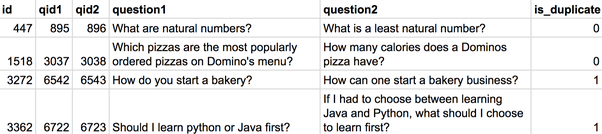
\includegraphics[width = 5in]{images/questions.png}
	\caption{Few sample lines of the quora dataset} %figure name
	\label{questions} % for referencing
	\source{https://data.quora.com/First-Quora-Dataset-Release-Question-Pairs}
\end{center}
\end{figure}

In figure \ref{questions} though the questions with qid1 and qid2 of 6542 and 6543 respectively mean the same, the phrase are completely different and hence are the duplicate questions. The existence of duplicate questions can be analyzed using the machine learning and training them using the datasets.\par
Unlike the first one, the questions with qid1 and qid2 of 895 and 896 respecively shown in figure \ref{questions} look similar in terms of phrases but are not the duplicates. We need to test for exact semantic coincidence between questions and analyze if it is the question with same intent.

\section{Problem Statement}
All the forums are based on the principle that ensures, each unique question exists on the forum only once and that there should be a single question section for each logically distinct question.  For example, we'd consider questions like ``What are the best ways to lose weight?'', ``How can a person reduce weight?'' and ``What are effective weight loss plans?'' to be duplicate questions because they all have the same intent and should not exist separately because the intent behind both is identical.\par

The duplication of questions in Q\&A Forums results in the lack of sensible search for the user base. A dull redundancy in the questions and answers still result in inadequacy of responses to the questioners. Inappropriate segragation of the valid information stream and unwanted distribution of the user base on varying level of activity and intellect of answers while polluting the user's feed. 

%The problems resulted due to question duplication may be enlisted as:
%\begin{enumerate}
%\item Lack of a sensible search.
%\item Segregation of information.
%\item Dull Redundancy but inadequacy of response to questioners.
%\item Distribution of user based on varying level of activity and intellect of answers.
%\end{enumerate}

\section{Objectives}
\begin{enumerate}
\item To develop a module to analyze and identify the questions having same semantic meaning so as to prevent the duplication for Q\&A forums like Quora .
\item To develop a module that would assist mitigatation of redundancy in answers to support high-quality knowledge base.
\end{enumerate}

\section{Applications}
Ideally, using this approach, the indentified duplicate questions could be merged together into a single canonical question, as doing so would provide a number of usage.  
\begin{enumerate}
	\item Avoid frequently repeated questions from polluting highly engaged user's feed on Q\&A forums caused by slight variations on the same questions.
	\item Improve search and discovery based on knowlegde of alternative phrasings of the same questions.
	\item High quality Q\&A knowledge bases having more value to users and researchers when there is a single cannonical question and colections of answers, instead of having knowledge fragmented and spread throughout the site.
\end{enumerate}


\section{Features}
\begin{enumerate}
\item Deep Learning to classify whether question pairs are duplicates or not.
\item Selected highly dominant features from the questions and implementation of minimal cost machine architectural model.
\end{enumerate}


\section{Feasibility Analysis}
\subsection{Economic Feasibility}
The economic feasibility determined from the nominal research shows positive economic benefits to the related institution that the system will provide. It involves cost/benefits analysis and it is the most frequently used method for evaluating the effectiveness of a new proposed system. Our project has requirements of software and hardware at medium level on implementation, that means it does not have a high economic requirement and is economically feasible to us, even at a nominal expense.
\par

\subsection{Technical Feasibility}
The technical feasibility studied the technical requirements that are to be taken under consideration in order to know if the proposed system is feasible or not. The technical area related to hardware and software requirements, requires not much of software nor hardware, and ultimately, it can be considered technically feasible.
\par

\subsection{Operational Feasibility}
Operational feasibility that accounts for our developed system has no demand for expert human resources. Considering the simplicity of our program, and the machine model obtained from it, we are assured that our project is operationally feasible to any area of application.


\section{System Requirements}
\subsection{Software Requirements}
Python is the choice for analyzing large volumes of data, processing it and implementing it for machine learning, with a large community for support and simplicity.
\begin{itemize}
\item \textbf{Development platform:} Python 3.7 or higher
\item \textbf{Operating System:} Windows 7, Ubuntu 16.04
\item \textbf{Integrated Development Environment:} Jupyter Notebook, Spyder
\item \textbf{Python Libraries:} keras, matplotlib, fuzzywuzzy, scikit-learn, nltk, numpy, pickle, pandas, flask 
\end{itemize}

\subsection{Hardware Requirements}
\begin{itemize}
	\item \textbf{RAM:} 8 GB RAM (Minimum)
	\item \textbf{Processor:} Intel Core i5-7th Generation
	\item \textbf{Storage:} 10 GB
\end{itemize}


\chapter{Literature Review}
In the paper `A Paraphrase and Semantic Similarity Detection System for User Generated Short-Text Content on Microblogs', a set of features was proposed that, although well-known in the NLP literature for solving other problems, had not been explored for detecting paraphrase or semantic similarity, on noisy user-generated short-text data such as Twitter. Support vector machine (SVM) based learning was applied and used the benchmark Twitter paraphrase data, released as a part of SemEval 2015, for experiments. The system delivered a paraphrase detection F1-score of 0.717 and semantic similarity detection F1-score of 0.741, thereby significantly outperforming the then-existing systems, that deliver F1-scores of 0.696 and 0.724 for the two problems respectively.\cite{Dey2016APA}
The main contributions of the work are the following:
\begin{itemize}
 \item It provided a machine learning based model, and a set of lexical, syntactic, semantic and pragmatic features, for detecting paraphrases on user-generated noisy Twitter short-text content data.
 \item Empirically showed the goodness of the proposed features, on a benchmark Twitter paraphrase corpus. The system outperformed all the systems that existed in the state of the art.
 \item Further demonstrated the effectiveness of the feature set on benchmark clean-corpus text data, namely Microsoft Paraphrase dataset, and obtain a rank within the top 10 existing systems, by training the system (the features) on their dataset, and testing on their dataset as well.
\end{itemize}

\textbf{Features Selection}
\begin{itemize}
	\item \textbf{Lexical Features :} Word-level gram features, Stemming, Stopword removal etc.
	\item \textbf{Syntactic Features: } Part-of-Speech (POS) agreement features, Named entity (NE) features
	\item \textbf{Semantic Features: } Word overlap features (Best word, Adjectives), Phrase overlap features 
	\item \textbf{Pragmatic Features: } Subjectivity/objectivity agreement feature
\end{itemize}

\textbf{Choice of Approach: Why not Deep Learning?} \\
This approach used the traditional methodology of identifying features, and a traditional SVM classifier. The choice
of modeling in the given manner was, in the known state of the art, traditional feature-based systems, had so far outperformed deep learning systems, such as the recurrent neural network based approaches for paraphrase detection. A deeper subsequent study also models deep neural learning systems, and observed a similar shortcoming of such systems.
A likely cause of this anomaly is the simple absence of a sufficiently large paraphrase dataset in the
domain of user-generated noisy texts on microblogs such as Twitter.

In the paper `Duplicate Quora Questions Detection' \cite{Guo2017DuplicateQQ} the main idea was to first vectorize questions and extract features, train and predict using machine learning techniques based on question vectors and features previously built. They implemented two approaches to detect if two questions are duplicate. Different vectorization and feature extracting methods were used in the two approaches, one based on the Word2Vec model and \ac{TFIDF} score, the other one is a Neural Network method based on term frequency. Different classification methods were also used, for example, \ac{KNN}, \ac{SVM} and Random Forest. This reached accuracies of nearly 80\% in both two approaches.

Using a dataset of 400,000 labeled question pairs provided by Q\&A forum Quora, researcher at Department of Computer Science, Stanford University explored a series of deep learning methodologies for detecting duplicate question pairs: convolutional neural networks (CNNs), long short-term memory networks (LSTMs), and a hybrid model\cite{Addair2017DuplicateQP}. All three models are built atop a siamese network architecture and multilayer perceptron concatenation for the final inference. Empirical results show that LSTMs outperform CNNs in terms of accuracy, and that combining the two techniques provides no additional inference improvements. Moreover, all three deep learning techniques significantly outperform traditional NLP methods and simple multilayer perceptron baselines.

Each question was passed into a separate tower of the network with identical parameters and weights, producing a “siamese network”. The raw questions, represented as single-dimensional vectors of vocabulary indexes, are then converted into pre-trained word in the embedding layer. The embedding matrix for each question is then passed through the encoding layer, that converts the word matrix into a single-dimensional feature vector. The feature vectors from each of the two
independent networks are concatenated together. Finally, the concatenated feature vectors are passed through a \acl{MLP} that produces the final output.
\begin{figure}[H]
\begin{center}
	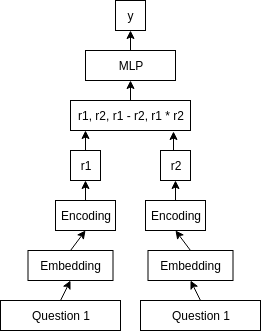
\includegraphics[width = 3in]{images/MLP.png}
	\caption{Siamese neural network architecture}
\end{center}
\end{figure}
Three different encoding strategies are used in the study in the encoding layer indicated in the figure above. Common to all three encoding methods is the final multilayer perceptron that combines the siamese network feature vectors together. The input to this network, when introduced, provided a 2\% performance gain over a simple concatenation of the
two feature vectors. Specifically, input used:
\begin{center}
\textbf{ (r1, r2, r1 - r2, r1 .* r2)}
\end{center} 
Where r1 and r2 are the output feature vectors from the first question and the second question, respectively. The third concatenated vector is the difference between the first and the second vectors (which will ultimately be symmetric given that each tower in the network uses the same model weights). Finally, the third concatenation is the element-wise
product between the first and second vectors.

ReLU activation was used for nonlinearity, and the final output layer consists of a single (1 x 2) vector, with the two
elements corresponding to each of the two classes: non-duplicate and duplicate.

In running experiments, a sample batch size of 64 was used and trained for a total of 20 epochs. Adam optimization was used with a learning rate of 0.001. Softmax cross entropy with logits was chosen for the loss. All of the implementation was written in TensorFlow, with separate run scripts for training and evaluation. Across all three of the models studied, a similar pattern of convergence was found. The model accuracy would sharply increase over the first training epoch, then quickly flatline after about 2 to 3 epochs.A similar pattern in the loss was observed, where it decreases for the first few epochs, then begins to increase consistently as the magnitude of the weights increases. 

Overall, it was found that the three deep learning models significantly out-performed the baselines across all metrics, but none of the three deep learning models stood out as being noticeably more expressive than the others. The \ac{LSTM} was notable for having slightly better overall performance than the \ac{CNN}, but being significantly faster to train and perform inference. Most surprising was that the hybrid model did not provide any gain in performance over the
\ac{LSTM} whatsoever, and in some ways may have actually underperformed it. It’s possible that the encoding of the LSTM captured some amount of information that was otherwise lost during \ac{CNN} filtering process.


Evaluation for extracting various features carried out which includes the concept of fuzzywuzzy and vector distances of the texts was hugely inspired from the presentation in Pydata, Berlin, Germany by Abhishek Thakur, regarding the Deep learning model\cite{AbskThakur} used in Question duplication analysis.

\chapter{Methodology}
\section{System Architecture and Overview}
The overall architecture of our system is show below. For each question in the pairs, the system undergoes a series of data preprocessing, feature extraction and engineering steps. The features from the question pairs are fed into a feed forward neural network for training and testing the accuracies. Similarly, the resulting trained model is used to evaluate a new pair of questions, following the same set of procedures of preprocessing, feature extraction and engineering to test for duplication.

\begin{figure}[H]
\begin{center}
	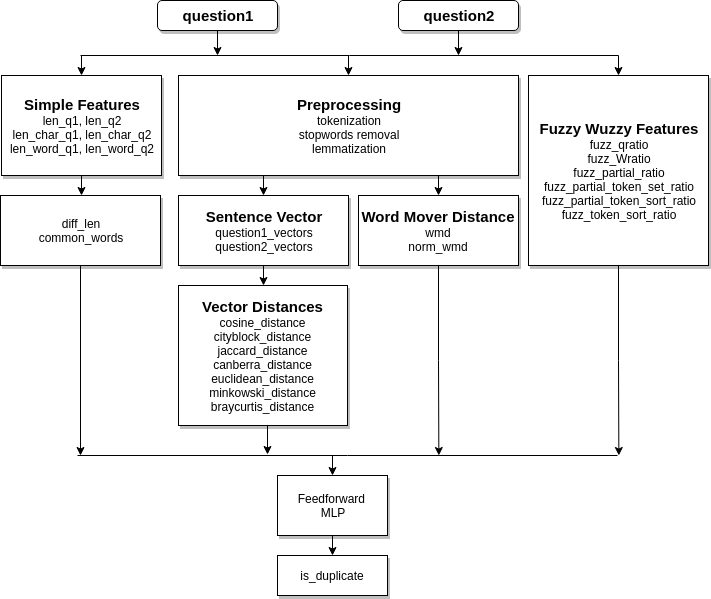
\includegraphics[width = 5.7in]{images/arch.png}
	\caption{Overall System Architecture.}
\end{center}
\end{figure}


\section{Data Acquisition and Dataset Description}
Quora has given an (almost) real-world dataset\cite{dataset} consising of a total of 404,290 question pairs in a tab-separated format; 255045 negative samples (non-duplicates) and 149306 positive samples (duplicates)  with the label of \textit{is\_duplicate} along with every question pair. Positive samples comprises 40\% of the total question pairs.

Target datasets can be downloaded from Quora. The training dataset contains valid question pairs , with labels: 
\begin{itemize}
	\item \textbf{id:} unique identifier for the question pair
	\item \textbf{qid1:} unique identifier for the first question
	\item \textbf{qid2:} unique identifier for the second question
	\item \textbf{question1:} full unicode text of the first question 
	\item \textbf{quesition2:} full unicode text of the second question 
	\item \textbf{is\_duplicate:} label 1 if questions are duplicates, 0 otherwise 
\end{itemize}
As a comparison, the test dataset contains 20\% of the total question pairs, but without any ``is\_duplicate'' label as a dataset for conducting further predictions on. The dataset was analyzed and the distribution was visualized in a count plot.
\begin{figure}[H]
\begin{center}
	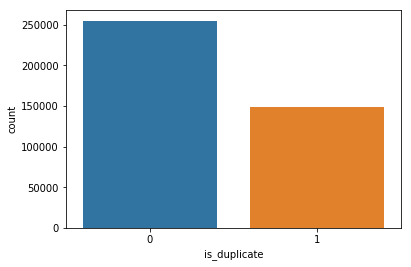
\includegraphics[width = 3.55in]{images/count.png}
	\caption{Distribution of the total question pairs.}
\end{center}
\end{figure}

\section{Data Pre-processing}
Insignificant columns; `id', `qid1', `qid2' are dropped from the dataset since these have no contibution in the learning the semantics of the questions. \textbf{Tokenization} and \textbf{lemmatization} are performed for each question on the dataset. Similarly, question mark (?) and all the \textbf{stops words} in the dataset are removed.

\subsection{Word Tokenization}
Word tokenization is the process of splitting a large sample of text into words. This is a requirement in natural language processing tasks where each word needs to be captured and subjected to further analysis like classifying and counting them for a particular sentiment etc.

\begin{figure}[tbh]
\begin{center}
	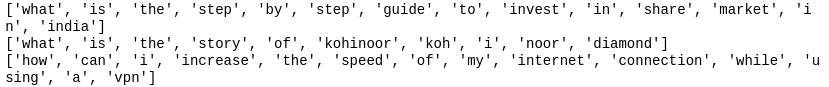
\includegraphics[width = 5.5in]{images/tokenization.png}
	\caption{Few questions after tokenization}
	\label{tokenization}
\end{center}
\end{figure}

\subsection{Stopwords}
A stop word is a commonly used word (such as “the”, “a”, “an”, “in”) that a search engine has been programmed to ignore, both when indexing entries for searching and when retrieving them as the result of a search query. We would not want these words taking up space in our database, or taking up valuable processing time. For this, we can remove them easily, by storing a list of words that you consider to be stop words. \ac{NLTK} in python has a list of stopwords stored in 16 different languages.
\begin{figure}[tbh]
\begin{center}
	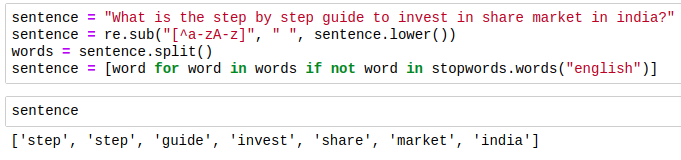
\includegraphics[width = 5.5in]{images/stopwords.png}
	\caption{A question after stopword removal}
	\label{stopwords}
\end{center}
\end{figure}

\subsection{Stemming and Lemmatization}
For grammatical reasons, documents are going to use different forms of a word, such as organize, organizes, and organizing. Additionally, there are families of derivationally related words with similar meanings, such as democracy, democratic, and democratization. In many situations, it seems as if it would be useful for a search for one of these words to return documents that contain another word in the set.

The goal of both stemming and lemmatization is to reduce inflectional forms and sometimes derivationally related forms of a word to a common base form. For instance:

\begin{figure}[tbh]
\begin{center}
	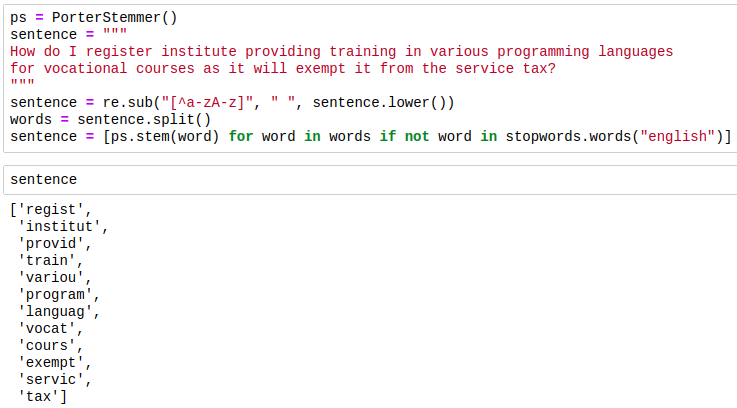
\includegraphics[width = 5.5in]{images/stem.png}
	\caption{A question after stopword removal and stemming}
	\label{stopwords}
\end{center}
\end{figure}
\newpage
\begin{figure}[tbh]
\begin{center}
	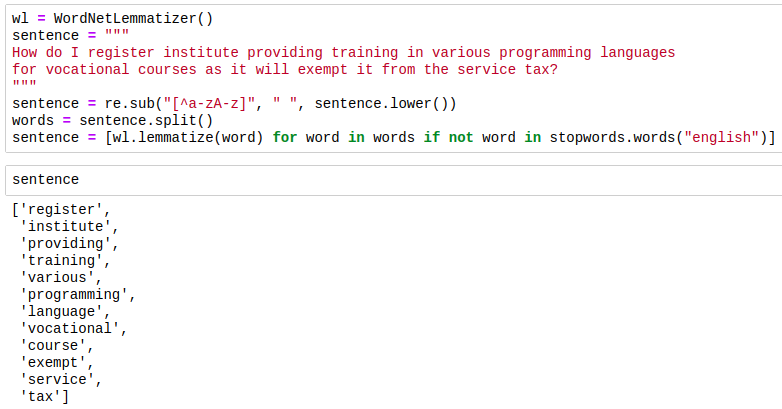
\includegraphics[width = 5.5in]{images/lemma.png}
	\caption{A question after stopword removal and lemmatization}
	\label{stopwords}
\end{center}
\end{figure}


\section{Feature Extraction}
The Machine Learning models as anticipated, is going to take in a lot of numerical values and vectors. For example, the number of times a word appears in a piece of text can be considered a feature. Several features are derived from the input text, and aggreggated on a per-text basis into feature vectors through Vector Space Modelling. Vector Space Modelling can largely be implemented via following techniques:

\subsection{Traditional Bag of Words}
A bag-of-words model is a way of extracting features from the text for the use in modeling. It is called a “bag” of words, because information about the order or structure of words in the document is discarded. This is only concerned with whether the known words occur in the document, not where in the document. Here, the length of document vector is equal to number of known words (vocabulary). 

\begin{figure}[tbh]
\begin{center}
	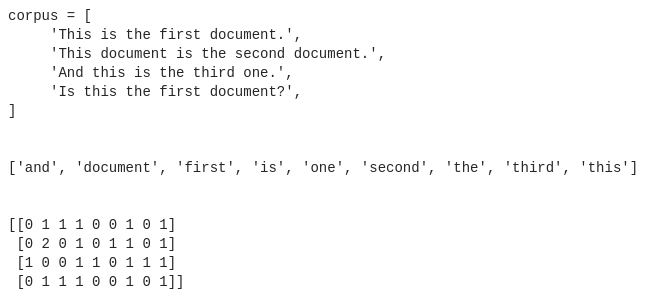
\includegraphics[width=5.5in]{images/bagofwords.png}
	\caption{Bag of words model for a small corpus.}
	\label{some_tfidf}
\end{center}
\end{figure}

\newpage

\subsection{Term Frequency Inverse-Document Frequency}
\ac{TFIDF} \cite{Ramos_usingtf-idf} is a reflect how important a word is to a document in a collection or corpus. One approach is to rescale the frequency of words by how often they appear in all the documents. Frequent words like is, a, the, etc are penalized. This approach to scoring is called Term Frequency–Inverse Document Frequency, where: 

\[W_i,_j = tf_i,_j * \log\frac{N}{df_i}\]

Where:
\begin{itemize}
    \item $tf_{i},_{j}$: number of occurance of $i$ in $j$
    \item $df_{i}$: is the number of documents containing $i$
    \item $N$: is the total number of documents
\end{itemize}


\begin{figure}[tbh]
\begin{center}
	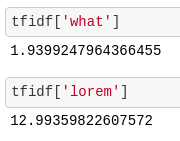
\includegraphics[width = 1.5in]{images/some_tfidf.png}
	\caption{\ac{TFIDF} of words 'what' and 'lorem'}
	\label{some_tfidf}
\end{center}
\end{figure}

\begin{itemize}
\item Term Frequency: It is the scoring of the frequency of the word in the document.
\item Inverse Document Frequency: It is the scoring of how rare the words are across the current documents.
\end{itemize} 

\subsection{Word Embedding: word2vec}
Word embedding is a collective name for a set of feature learning techniques and language modeling in Natural Language Processing. Here words and phrases are mapped into vectors of real numbers. These models are shallow, two-layer neural networks that are trained to reconstruct linguistic contexts of words. Word2vec \cite{DBLPRong14} takes input a very large corpus of text and produces a vector space, which consist of several hundred dimensions, with each unique word in the corpus assigned equivalent vector in the space. Word vectors are positioned in the corresponding vector space such that words that share common contexts in the body are located in near to one another in the space. 

\subsubsection{Continuous Bag of Word Model}
\ac{CBOW} is learning to predict the word by the context. A context may be single word or multiple word for a given target words. Lets see this by an example “The cat jumped over the puddle.” So one approach is to treat {“The”, “cat”, ’over”, “the’, “puddle”} as a context and from these words, be able to predict or generate the center word “jumped”. This type of model we call a Continuous Bag of Words  Model.

\subsubsection{Skip-gram Model}
Another approach is to create a model such that given the center word “jumped”, the model will be able to predict or generate the surrounding words “The”, “cat”, “over”, “the”, “puddle”. Here we call the word “jumped” the context. We call this type of model a SkipGram model.


\clearpage
\begin{figure}[tbh]
\begin{center}
	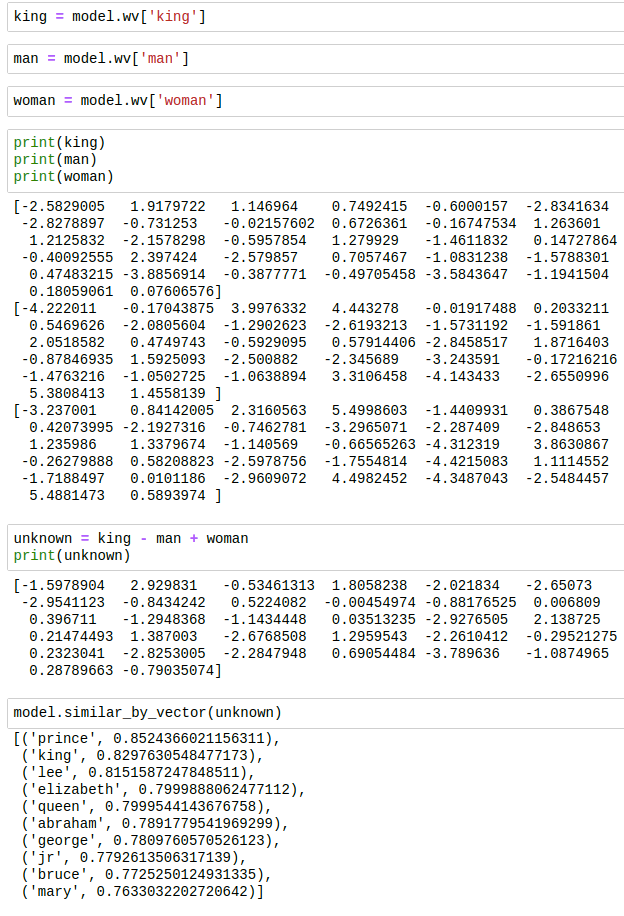
\includegraphics[width = 4.55in]{images/word2vec_.png}
	\caption{Word2vec model showing similar words of an unknown vector with semantic context}
	\label{some_tfidf}
\end{center}
\end{figure}	


\newpage
\begin{figure}[tbh]
\begin{center}
	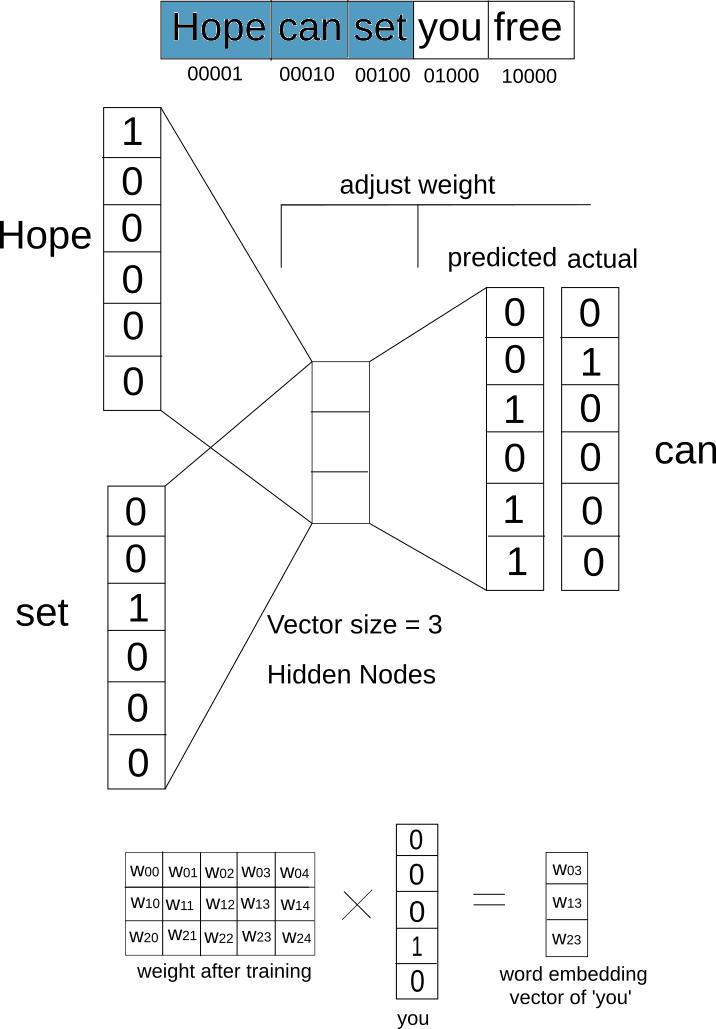
\includegraphics[width = 4.5in]{images/cbow.png}
	\caption{CBOW model}
	\label{cbow}
\end{center}
\end{figure}

	
\subsection{Google News vectors}
	The repository provided by the Google consist of word2vec pre-trained Google News corpus word vector model which consists of 3 million 300  dimension English word vectors. Google News Vector includes word vectors for a vocabulary of 3 million words and phrases that are trained on around 100 billion words from a Google News dataset. We require a high amount of memory to process this because gensim allocates a big matrix to hold all of the word vectors, and if we do the math, this is a huge matrix. Mathematically, 3 million words * 300 features * 4bytes/feature = ~3.35GB
	

\section{Feature Engineering}
Feature engineering involves extracting of information from the given dataset. Features are divided into four categories. This involves the working of basic \textit{NLTK mathematics}, \textit{fuzywuzzy parameters}, \textit{Word Mover Distance} and \textit{Vector distance}.

\subsection{NLTK Library Groundworks}
The simple features: \textit{len\_q1, len\_q2, diff\_len, len\_char\_q1, len\_char\_q2, len\_word\_q1, len\_word\_q2 and common\_words} are derived from the dataset.

\begin{figure}[tbh]
\begin{center}
	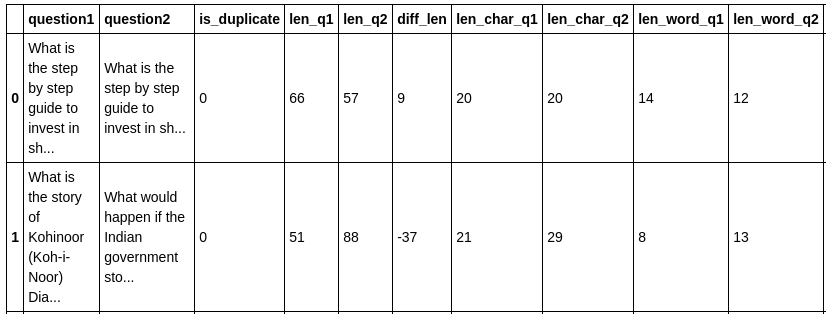
\includegraphics[width = 5.2in]{images/features_I.png}
	\caption{Simple feature extraction.}
	\label{features_I}
\end{center}
\end{figure}

\subsection{ Fuzzy wuzzy Features }
Fuzzy String Matching is sometimes known as approximate string matching. It is the process of finding strings that approximately match a given pattern. It uses Levenshtein Distance to calculate the differences between sequences in a simple-to-use package. \textbf{The closeness of a match is measured in terms of edit distance, which is the number of primitive operations (insertion, deletion and substitution) necessary to convert the string into an exact match.} \textit{ Fuzzy QRatio, Fuzzy WRatio, Fuzzy partial ratio, Fuzzy partial token set ratio, Fuzzy partial token sort ratio, Fuzzy token set ratio and Fuzzy token sort ratio} are extracted from the questions pairs.

\begin{table}[]
\begin{center}
\begin{tabular}{|l|l|l|}
\hline
\textbf{Simple Ratio}     & \textit{``this is a test", ``this is a test!"}                           & 97  \\
\hline
\textbf{Partial Ratio}    & \textit{``this is a test", ``this is a test!"}                   & 100 \\ \hline
\textbf{Token Sort Ratio} & \textit{``fuzzy wuzzy was a bear", ``wuzzy fuzzy was a bear"} & 100 \\ \hline
\textbf{Token Set Ratio}  & \textit{``fuzzy was a bear", ``fuzzy fuzzy was a bear"}        & 100 \\ \hline
\end{tabular}
\end{center}
\caption{Fuzzy Wuzzy sample features}
\end{table}

\begin{figure}[tbh]
\begin{center}
	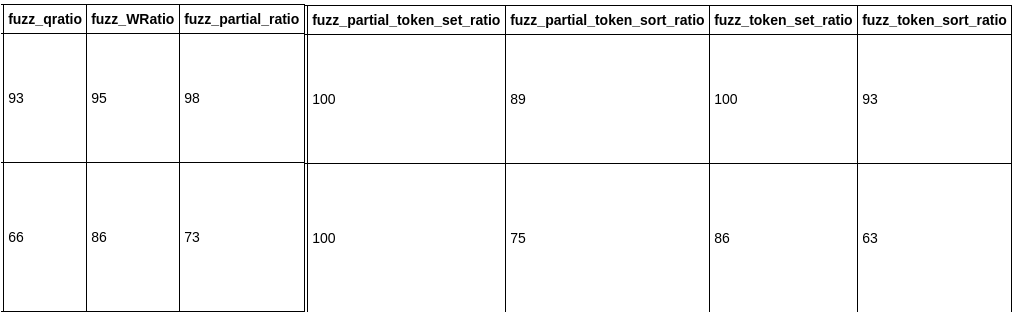
\includegraphics[width = 5.2in]{images/features_II.png}
	\caption{Fuzzy feature extraction.}
	\label{features_I}
\end{center}
\end{figure}


\subsection{Word Mover Distance}
\ac{WMD} is a method that allows us to assess the distance between two texts, even when they have no words in common. It uses \textit{word2vec} vector embeddings of words. Normalized \ac{WMD}, on the other hand, uses the Euclidean distance for calculation. To use \ac{WMD}, we need some word embeddings. Gensim is very helpful for this purpose.

\subsection{Vector distances}
Various vector distances: \textit{Cosine, Cityblock, Canberra, Euclidean, Minkowski and Braycurti distances} are measured for all the question pairs. These distances are plotted against common words which gives the similar plot.

\subsubsection{Some Distance Metrics}
\begin{itemize}
	\item \textbf{Cosine Distance:} Cosine similarity is a measure of similarity between two non-zero vectors of an inner product space that measures the cosine of the angle between them.

	\[similarity = cos(\theta) = \frac{A.B}{|A||B|}=\frac{\sum_{i=1}^n A_{i}B_{i}}{ \sqrt{\sum_{i=1}^n A_{i}^2} \sqrt{\sum_{i=1}^n B_{i}^2} }\] \\
	
	
	\item \textbf{Euclidean Distance:} Euclidean distance is the `ordinary' straight-line distance between two points in Euclidean space.
	\[ d(p,q) = d(q,p) = \sqrt{(q_1-p_1)^2 + (q_2-p_2)^2 +.... + (q_n-p_n)^2} \]
	\[ \sqrt{\sum_{i=1}^n(q_n-p_n)^2} \] \\
	
	\item \textbf{Minkowski Distance:} The Minkowski distance is a metric in a normed vector space which can be considered as a generalization of both the Euclidean distance and the Manhattan distance. The Minkowski distance of order p between two points:
	\[D(X,Y) = (\sum_{i=1}^n | x_i - y_i | ^p )^{1/p}\]

\end{itemize}

\begin{figure}[tbh]
\begin{center}
	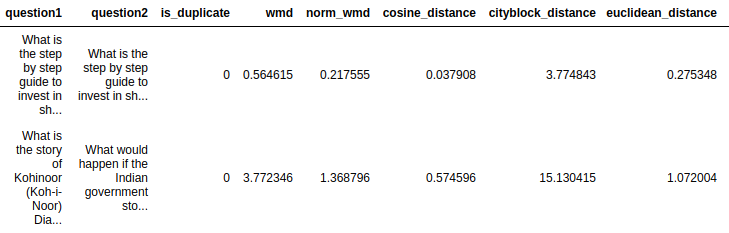
\includegraphics[width=5.5in]{images/vector.png}
	\caption{Some vector distances between questions in pair}
	\label{vector}
\end{center}
\end{figure}

\begin{figure}[tbh]
	\begin{center}
		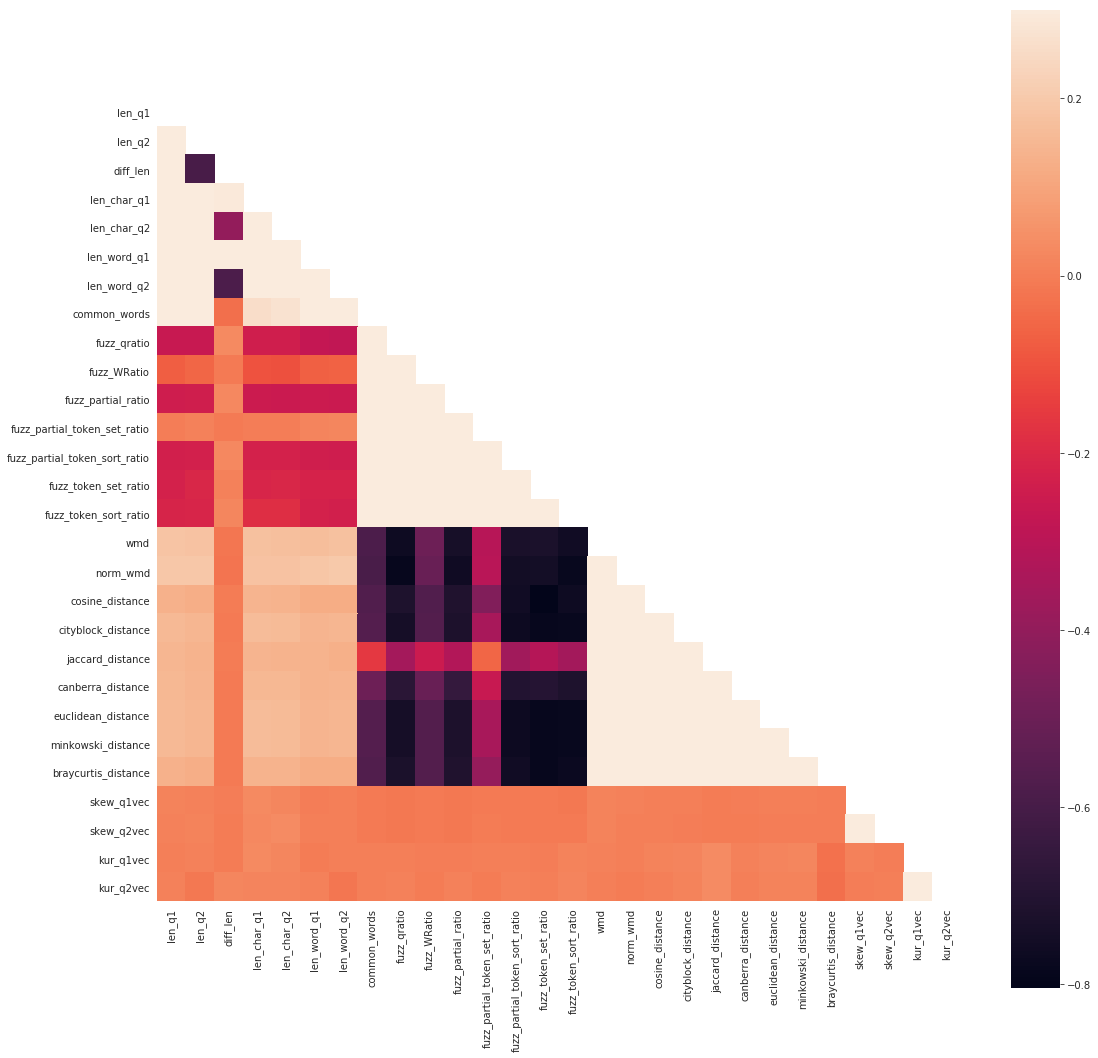
\includegraphics[width = 5.9in]{images/heatmap.png}
		\caption{Correlation Heatmap of features.}
		\label{heatmap}
	\end{center}
\end{figure}	

\par All the features were combined into a single space, and then, the mathematical implication was realized.

\clearpage
\section{Analysis and Visualization}
\begin{figure}[tbh]
\begin{center}
	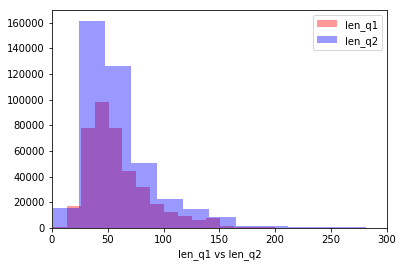
\includegraphics[width=4in]{images/len.png}
	\caption{Distribution of lengths of question pairs}
	\label{len}
\end{center}
\end{figure}

\begin{figure}[tbh]
\begin{center}
	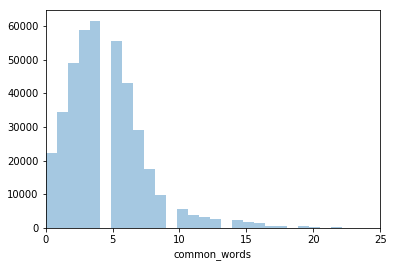
\includegraphics[width=4in]{images/common.png}
	\caption{Distribution of common words of question pairs}
	\label{common}
\end{center}
\end{figure}

\newpage
\begin{figure}[tbh]
\begin{center}
	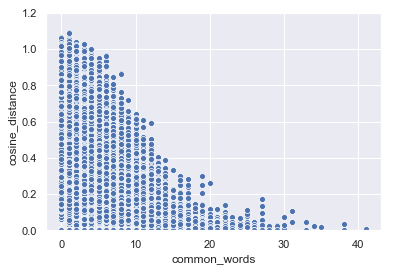
\includegraphics[width=4in]{images/scatter1.png}
	\caption{Scatter plot of common words and cosine distance of question pairs}
	\label{scatter1}
\end{center}
\end{figure}

\begin{figure}[tbh]
\begin{center}
	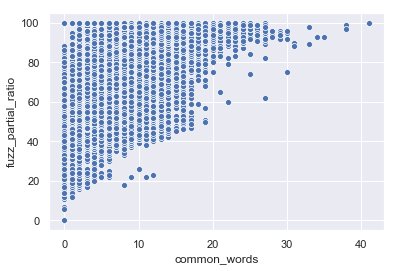
\includegraphics[width=4in]{images/scatter2.png}
	\caption{Scatter plot of common words and fuzz partial ratio of question pairs}
	\label{scatter2}
\end{center}
\end{figure}

\newpage

\section{Supervised Machine Learning Models}
For the validation of feature-engineered parameters, application of different supervised machine learning algorithms is possible along with the study of their accuracy and results for few parameters. The supervised machine learning algorithms under considerations via \textit{scikit-learn} library are:

\begin{table}[tbh]
\begin{center}
\begin{tabular}{|l|l|l|ll}
\cline{1-3}
\textbf{S.N.} & \textbf{Supervised Machine Learning} & \textbf{Accuracy} &  &  \\ \cline{1-3}
1             & Random Forest                        & 0.7235            &  &  \\ \cline{1-3}
2             & K Nearest Neighbors                  & 0.7104            &  &  \\ \cline{1-3}
3             & Logistic Regression                  & 0.6680            &  &  \\ \cline{1-3}
\end{tabular}
\caption{Comparison of Supervised models for duplication analysis}
\end{center}
\end{table}


\section{Neural Network Design}
Artificial neural networks (ANN) or connectionist systems are computing systems vaguely inspired by the biological neural networks and astrocytes that constitute animal brains. The neural network itself is not an algorithm, but rather a framework for many different machine learning algorithms to work together and process complex data inputs. Such systems "learn" to perform tasks by considering examples, generally without being programmed with any task-specific rules.

An ANN is based on a collection of connected units or nodes called artificial neurons, which loosely model the neurons in a biological brain. Each connection, like the synapses in a biological brain, can transmit a signal from one artificial neuron to another. An artificial neuron that receives a signal can process it and then signal additional artificial neurons connected to it.

In the brain, neurons can be connected to many other neurons nearby. In a typical neural network, however, information only flows one way. These neurons are spread across three layers:

\begin{enumerate}
\item The input layer consists of the neurons that do nothing more than receive the data and pass it on. The number of neurons in the input layer should be equal to the number of features in your data set.

\item The output layer consists of a number of nodes depending on the type of model you’re building. In a classification system, there will be one node for each type of label you might be applying, while in a regression system there will just be a single node that puts out a value.

\item In between these two layers is where things get interesting. Here, we have what’s called the hidden layer, which also consists of a number of neurons (how many will depend on the number of neurons in your input and output layers, but don’t worry about that). The nodes in the hidden layer apply transformations to the inputs before passing them on. As the network is trained, those nodes that are found to be more predictive of the outcome are weighted more heavily.
\end{enumerate}


	\begin{figure}[tbh]
	\begin{center}
		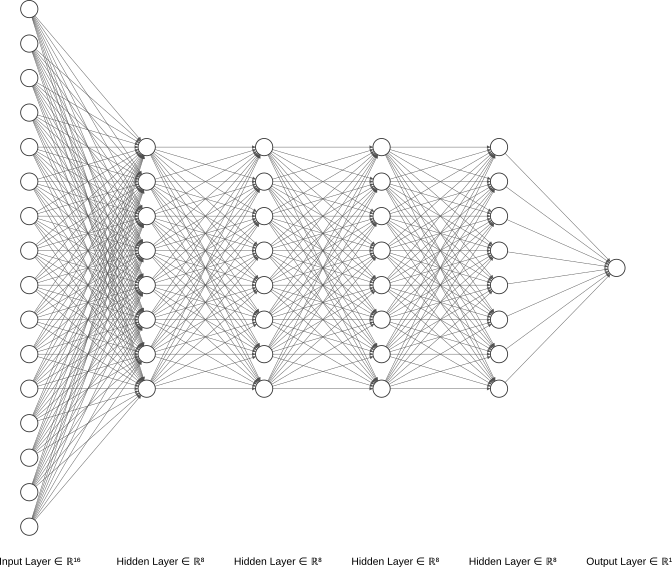
\includegraphics[width = 5in]{images/g719.png}
		\caption{Architecture of Neural Network}
		\label{neuralnetwork}
	\end{center}
	\end{figure}

\subsection{Framework of \acl{ANN}:}
\begin{enumerate}
	\item Assign random weights to all linkages to start the algorithm.
	\item Using inputs and the (input - hidden node) linkages, find the activation rate of the hidden nodes.
	\item Using activation rate of the hidden nodes and linkages to output, find the activation rate of output nodes.
	\item Find the error rate at the output node and recalibrate all the linkages between hidden nodes and output nodes.
	\item Using weights and error found at the output node, cascade down the error to hidden nodes.
	\item Recalibrate the weights between hidden node and the input nodes.
	\item Repeate the process till the convergence criterion is met.
	\item Using the final weights, score the activation rate of the output node.
\end{enumerate}

After completion of feature engineering, the parameters extracted are now tested to evaluate how these parameters affect the performance of our neural network. 16 best parameters are chosen through the analysis of correlation heat-map as show in figure \ref{heatmap}. Artificial Neural Network is designed consisting of 5 hidden layers. Input layer consists of 16 nodes that send information to the hidden layer. The exact artificial neural network of our model, consist of an input layer with 16 input nodes, 5 hidden layers with 8 nodes each for precise result calculation and a single output node that results 1 or 0 i.e. duplicate or not\_duplicate.

The nodes in the input layer and the hidden layers have \ac{ReLU} as the activation function, while the output node has sigmoid function as the activation fucntion.

Mathematically, \ac{ReLU} it is defined as y = max(0, x). Visually, it looks like the following:

\begin{figure}[tbh]
	\begin{center}
		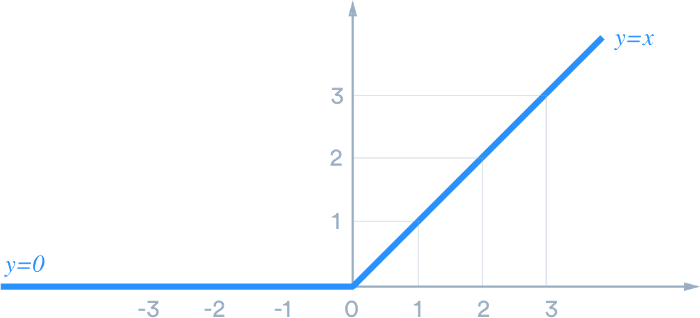
\includegraphics[width = 4in]{images/relu.png}
		\caption{ReLU activation function}
		\label{relu}
	\end{center}
\end{figure}

\ac{ReLU} is linear (identity) for all positive values, and zero for all negative values. This means that:

\begin{enumerate}
		\item It’s cheap to compute as there is no complicated math. The model can therefore take less time to train or run.
		\item It converges faster. Linearity means that the slope doesn’t plateau, or “saturate,” when x gets large. It doesn’t have the vanishing gradient problem suffered by other activation functions like sigmoid or tanh.
		\item It’s sparsely activated. Since ReLU is zero for all negative inputs, it’s likely for any given unit to not activate at all.
\end{enumerate}
	
	Many natural processes, such as those of complex system learning curves, exhibit a progression from small beginnings that accelerates and approaches a climax over time. When a specific mathematical model is lacking, a sigmoid function is often used.Often, sigmoid function refers to the special case of the logistic function shown in the figure \ref{sigmoid} and defined by the formula:	
	\[S(X) = \frac{1}{1+e^{-x}}	\]

	\begin{figure}[tbh]
	\begin{center}
		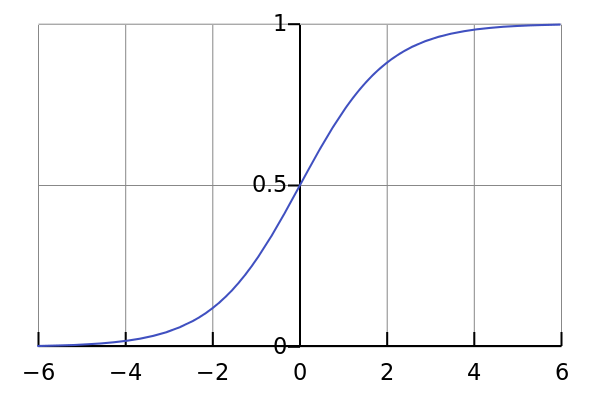
\includegraphics[width = 3.5in]{images/sigmoid.png}
		\caption{Sigmoid Activation Function}
		\label{sigmoid}
	\end{center}
	\end{figure}
	
\subsection{Adam optimization}
Adam is an optimization algorithm that can used instead of the classical stochastic gradient descent procedure to update network weights iterative based in training data. Stochastic gradient descent maintains a single learning rate (termed alpha) for all weight updates and the learning rate does not change during training. The method computes individual adaptive learning rates for different parameters from estimates of first and second moments of the gradients.
Adam can be looked at as a combination of Root Mean Square Propagation and Stochastic Gradient Descent with momentum. It uses the squared gradients to scale the learning rate like Root Mean Square Propagation and it takes advantage of momentum by using moving average of the gradient instead of gradient itself like Stochastic Gradient Descent with momentum.
\subsubsection{Adam Configuration Parameters}
\begin{itemize}
\item alpha. Also referred to as the learning rate or step size. The proportion that weights are updated (e.g. 0.001). Larger values (e.g. 0.3) results in faster initial learning before the rate is updated. Smaller values (e.g. 1.0E-5) slow learning right down during training
\item beta1. The exponential decay rate for the first moment estimates (e.g. 0.9).
\item beta2. The exponential decay rate for the second-moment estimates (e.g. 0.999). This value should be set close to 1.0 on problems with a sparse gradient (e.g. NLP and computer vision problems).
\item epsilon. Is a very small number to prevent any division by zero in the implementation (e.g. 10E-8).
\end{itemize}

\subsection{Training}
We used 20\% of dataset as testing dataset and remaining 80\% as training dataset. Input parameter are: diff\_len, common\_words, fuzz\_qratio ,fuzz\_WRatio, fuzz\_partial\_ratio, fuzz\_partial\_token\_set\_ratio, fuzz\_partial\_token\_sort\_ratio, fuzz\_token\_set\_ratio, \newline fuzz\_token\_sort\_ratio, wmd, cosine\_distance, cityblock\_distance, canberra\_distance, euclidean\_distance, minkowski\_distance and braycurtis\_distance. The batch size is 10 and 30 epochs are used for training of our model. Batch size defines the number of samples that are going to be propagated each time through the network.	

\begin{figure}[H]
\begin{center}
	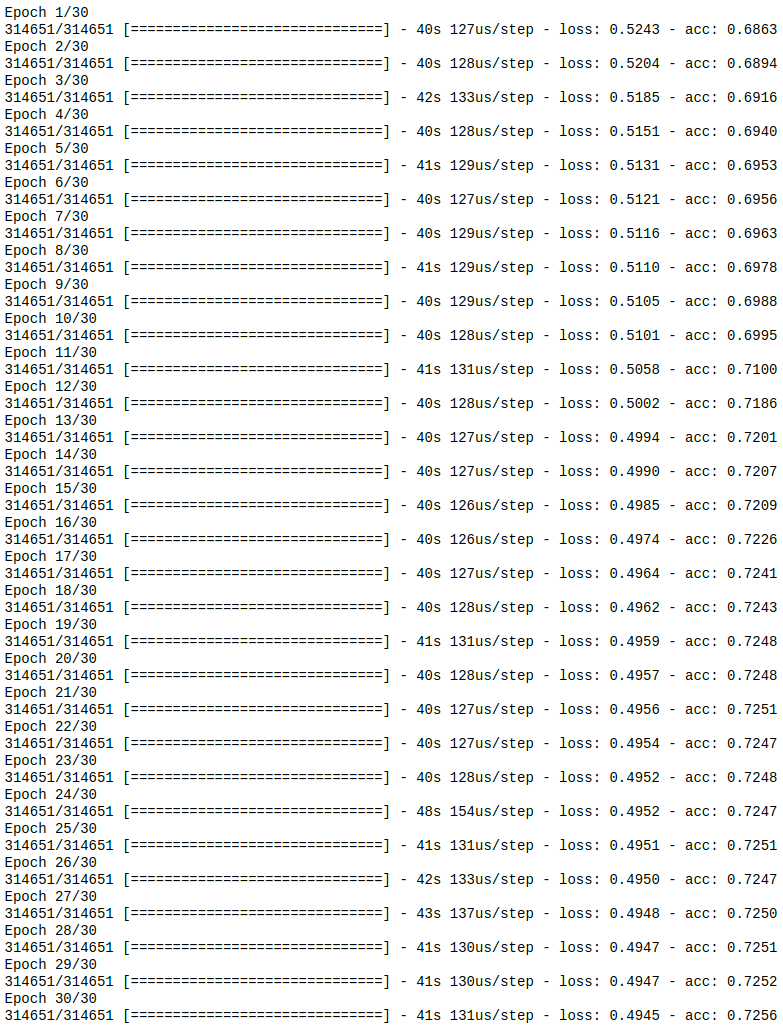
\includegraphics[width = 5in]{images/epoch.png}
	\caption{Training of \ac{ANN}} %figure name
\end{center}
\end{figure}	
	
\newpage	
	
\par
\section{Software Development Model}
Our development approach is based upon \textbf{`Test Driven Development'}, that relies on the repetition of a very short development cycle: our requirements such as feature extraction, feature engineering, model development are turned into very specific test cases, then the program is improved to pass the new tests of required results. \textit{This is opposed to software development that allows software to be added that is not proven to meet requirements.}

\begin{figure}[H]
\begin{center}
	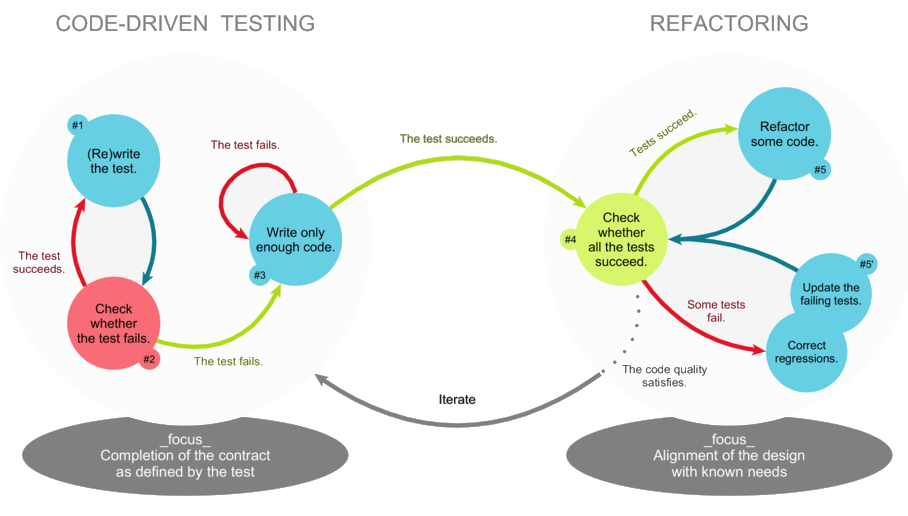
\includegraphics[width = 5.7in]{images/testdrivendevelopment.png}
	\caption{Test Driven Development Model} %figure name
	\source{https://en.wikipedia.org/wiki/Test-driven\_development}
\end{center}
\end{figure}

\subsection{Sequence based on Test-Driven Development by Example:}
\begin{enumerate}
	\item \textbf{Add a test:} \par In test-driven development, each new feature begins with writing a test. Write a test that defines a function or improvements of a function, which should be very succinct. To write a test, we as a developer must clearly understand the feature's specification and requirements.
	
\item \textbf{Run all tests and see if the new test fails:} \par This validates that the test harness is working correctly, shows that the new test does not pass without requiring new code because the required behavior already exists, and it rules out the possibility that the new test is flawed and will always pass. The new test should fail for the expected reason. This step increases the our confidence in the new test.	

\item \textbf{Write the code:} \par The next step is to write some code that causes the test to pass. The new code written at this stage is not perfect and may pass the test in an inelegant way. That is acceptable because it will be improved and honed in Step 5.

\item \textbf{Run tests: } \par If all test cases now pass, we can be confident that the new code meets the test requirements, and does not break or degrade any existing features. If they do not, the new code must be adjusted until they do.	
	
\item \textbf{Refactor code: } \par The growing code base must be cleaned up regularly during test-driven development. New code can be moved from where it was convenient for passing a test to where it more logically belongs. Duplication must be removed. Object, class, module, variable and method names should clearly represent their current purpose and use, as extra functionality is added.

\item \textbf{Repeat}		
	
\end{enumerate}


\chapter{Output}

\begin{figure}[tbh]
\begin{center}
	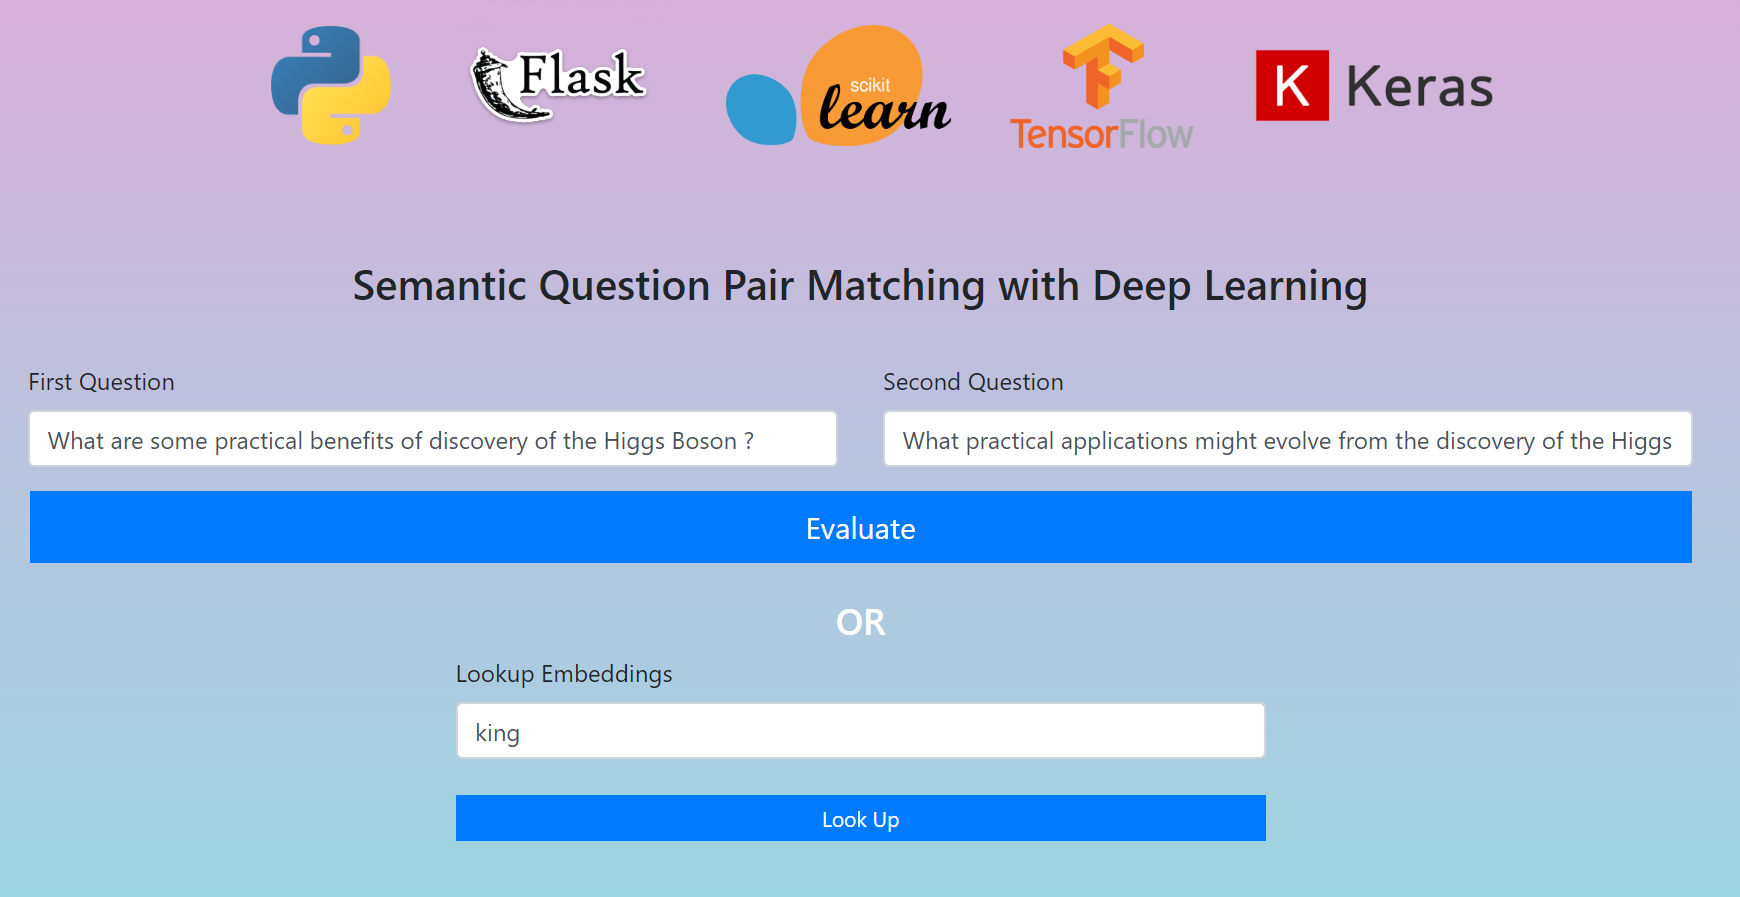
\includegraphics[width=5.85in]{images/outputs/home.png}
	\caption{Home page to evaluate a pair of questions or lookup similar words.}
	\label{home}
\end{center}
\end{figure}

\begin{figure}[tbh]
\begin{center}
	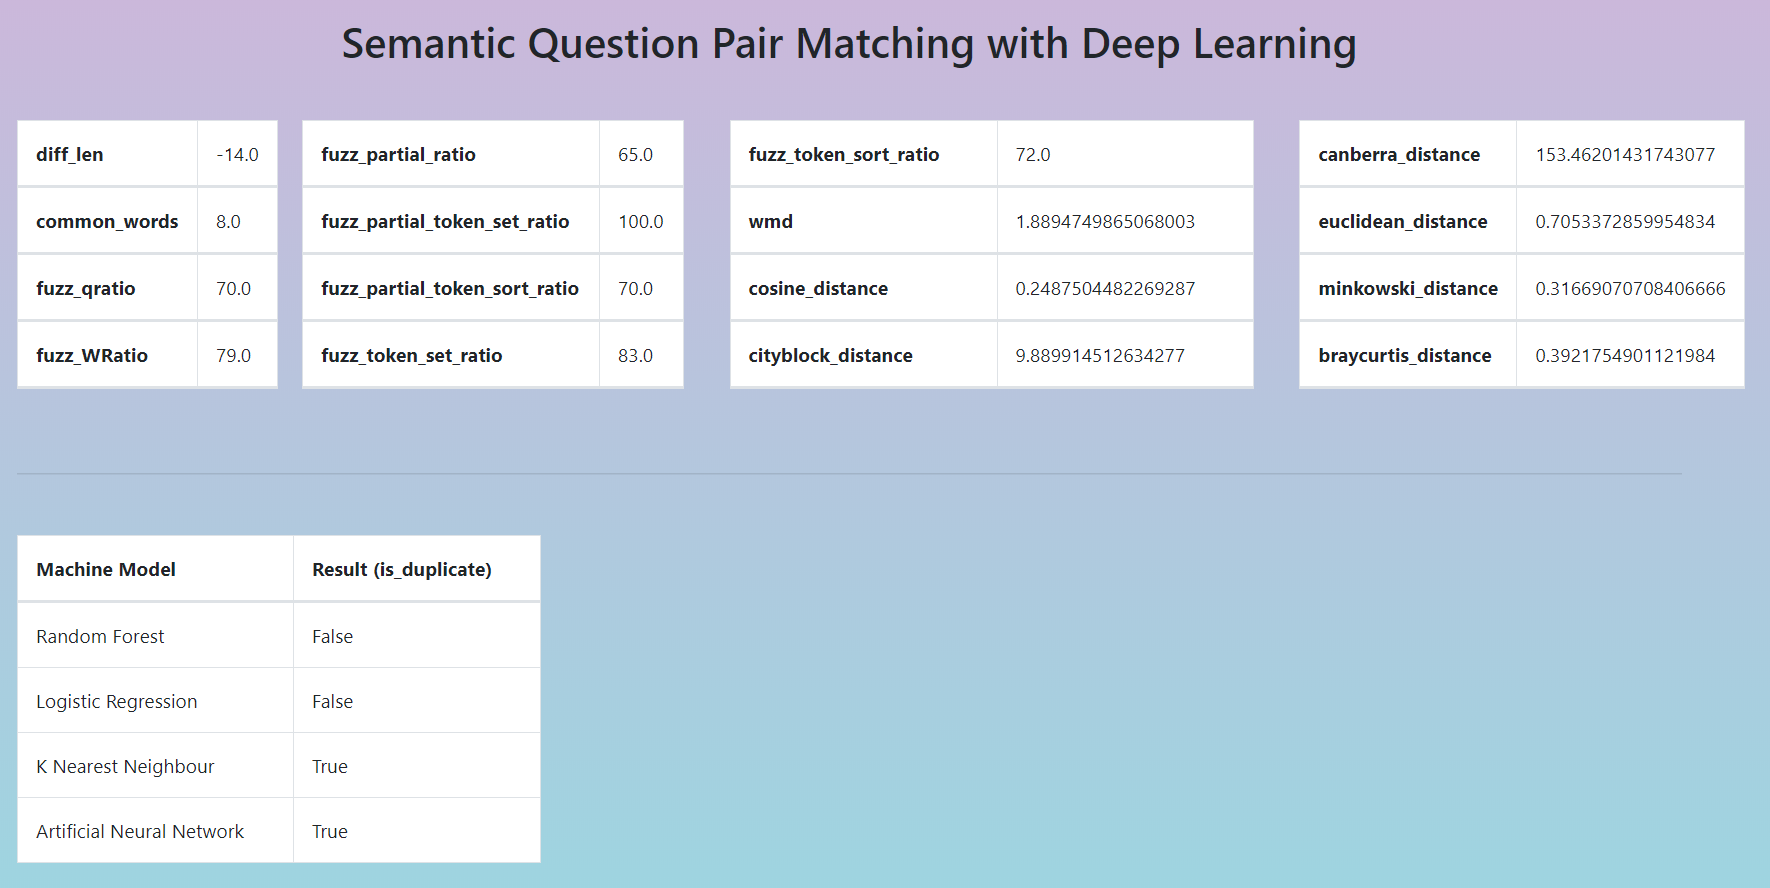
\includegraphics[width=5.85in]{images/outputs/evaluate.png}
	\caption{Evaluating a pair of questions.}
	\label{evaluate}
\end{center}
\end{figure}

\begin{figure}[tbh]
\begin{center}
	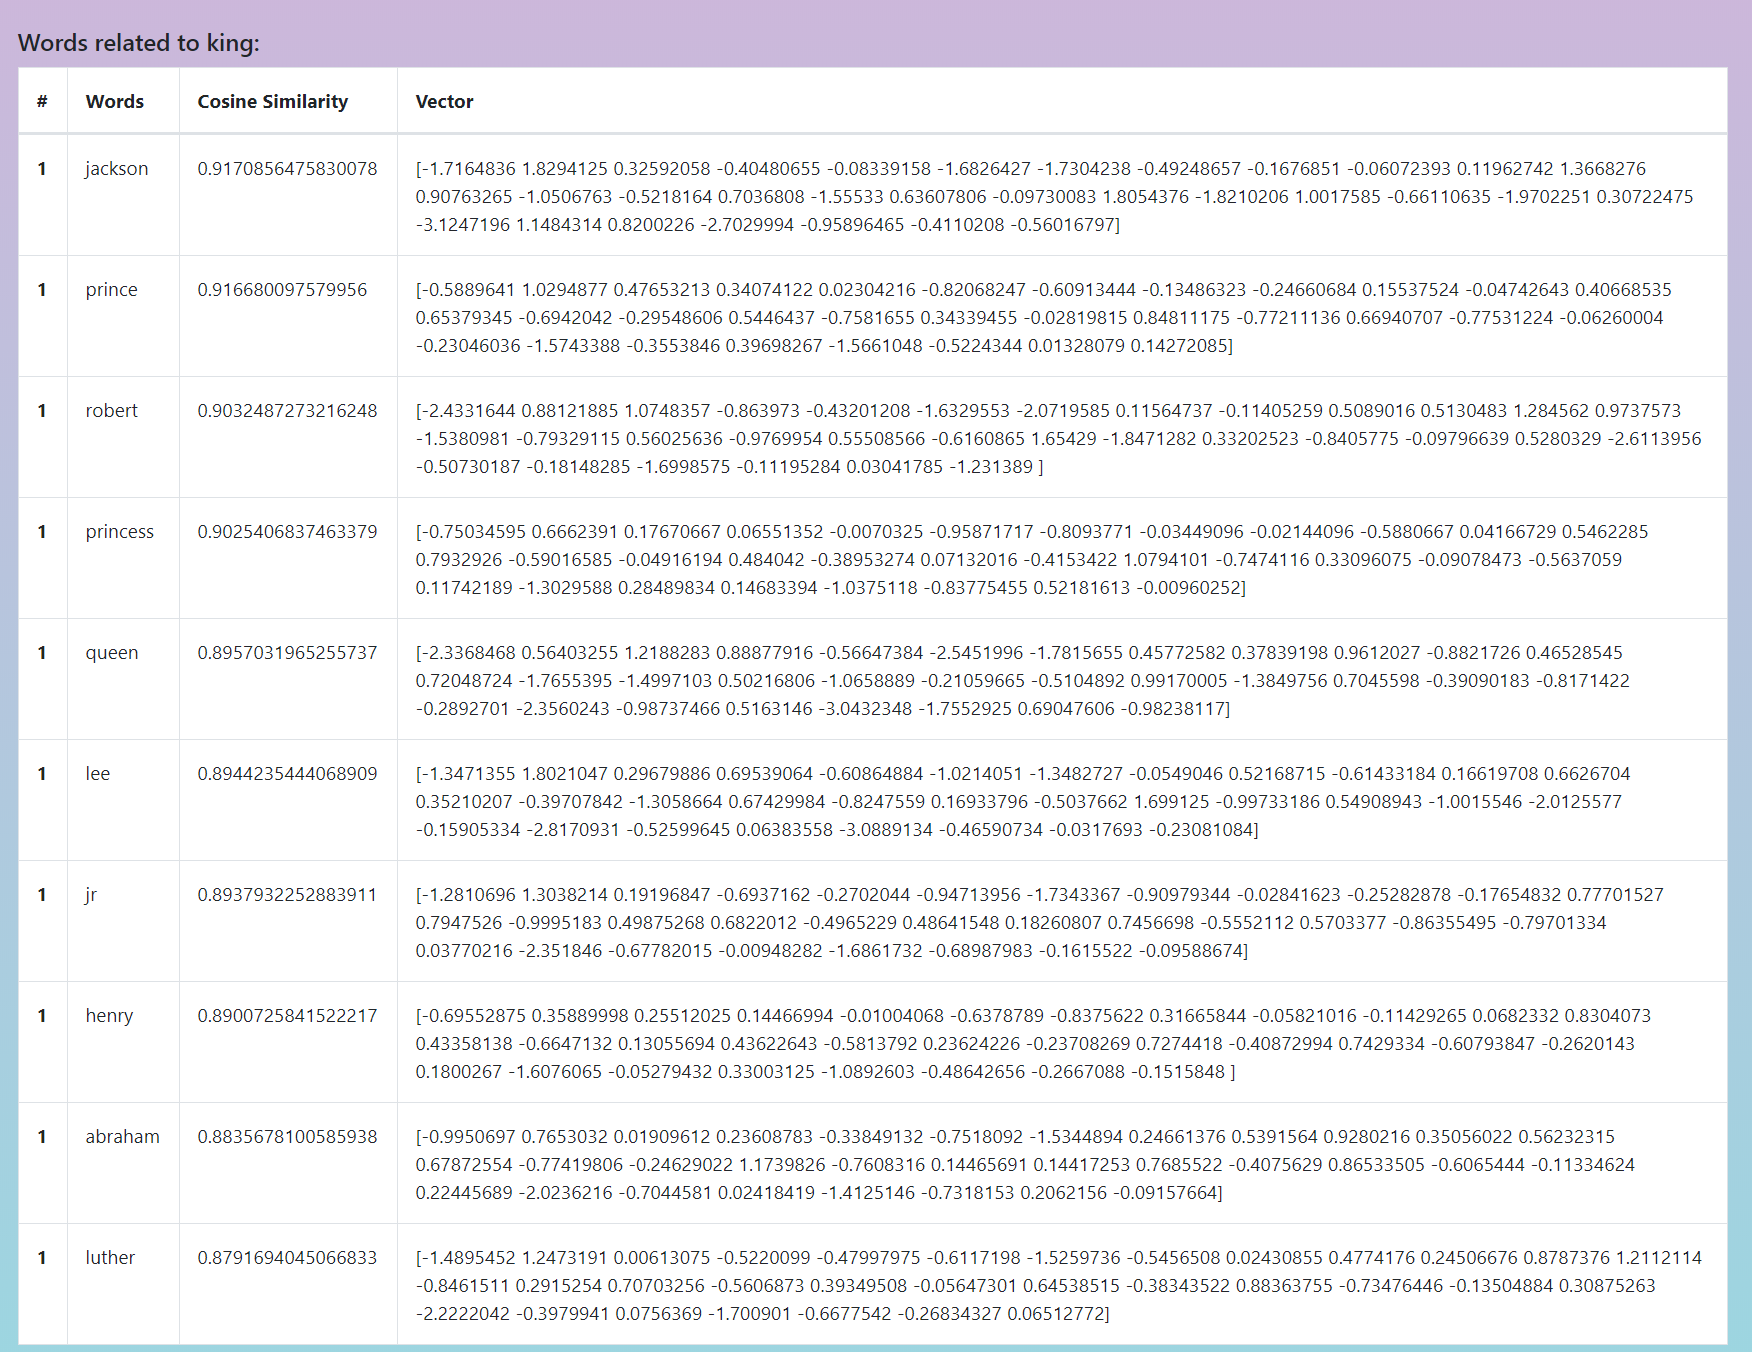
\includegraphics[width=5.85in]{images/outputs/lookup.png}
	\caption{Lookup similar words from word2vec model.}
	\label{lookup}
\end{center}
\end{figure}

\newpage
\chapter{Results and Analysis}
\section{Confusion Matrix}
A Confusion Matrix is a popular representation of the performance of classification models. The matrix (table) shows us the number of correctly and incorrectly classified examples, compared to the actual outcomes (target value) in the test data. One of the advantages of using confusion matrix as evaluation tool is that it allows more detailed analysis (such as if the model is confusing two classes), than simple proportion of correctly classified examples (accuracy) which can give misleading results if the dataset is unbalanced (i.e. when there are huge differences in number of between difference classes).

The matrix is n by n, where n is the number of classes. The simplest classifiers, called binary classifiers, has only two classes: positive/negative, yes/no, male/female… Performance of a binary classifier is summarized in a confusion matrix that cross-tabulates predicted and observed examples into four options:

\begin{itemize}
	\item True Positive (TP): Correctly predicting a label (we predicted “yes”, and it’s “yes”),
	\item True Negative (TN): Correctly predicting the other label (we predicted “no”, and it’s “no”),
	\item False Positive (FP): Falsely Predicting a label (we predicted “yes”, but it's “no”),
	\item False Negative (FN): Missing and incoming label (we predicted “no”, but it’s “yes”).
\end{itemize}

The corresponding table of confusion, for the duplicate and non-duplicate, would be as shown:

\begin{table}[tbh]
\begin{center}
\begin{tabular}{c|c|c|c|}
\cline{2-4}
\multicolumn{1}{l|}{}                                                                                   & \multicolumn{3}{c|}{\textbf{\begin{tabular}[c]{@{}c@{}}Predicted \\ Values\end{tabular}}} \\ \hline
\multicolumn{1}{|c|}{\multirow{3}{*}{\textbf{\begin{tabular}[c]{@{}c@{}}Acutal\\ Values\end{tabular}}}} & \multicolumn{1}{l|}{\textit{is\_duplicate}}           & 0               & 1               \\ \cline{2-4} 
\multicolumn{1}{|c|}{}                                                                                  & 0                                                     & 36462           & 12792           \\ \cline{2-4} 
\multicolumn{1}{|c|}{}                                                                                  & \textit{1}                                            & 8954            & 20455           \\ \hline
\end{tabular}
\end{center}
\caption{Corresponding Confusion Matrix of \ac{ANN} Model}
\end{table}

%\begin{figure}[H]
%\begin{center}
%	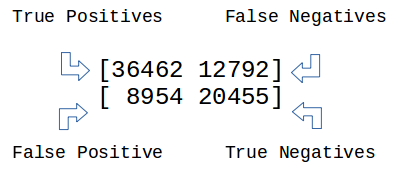
\includegraphics[width = 2.5in]{images/cm.png}
%	\caption{Corresponding Confusion Matrix} %figure name
%\end{center}
%\end{figure}

\begin{table}[tbh]
\begin{center}
\begin{tabular}{|c|c|c|}
\hline
\textbf{Measure}          & \textbf{Value} & \textbf{Derivations}       \\ \hline
Sensitivity               & 0.6955         & TPR = TP / (TP + FN)       \\ \hline
Specificity               & 0.7403         & SPC = TN / (FP + TN)       \\ \hline
Precision                 & 0.6152         & PPV = TP / (TP + FP)       \\ \hline
Negative Predictive Value & 0.8028         & NPV = TN / (TN + FN)       \\ \hline
False Positive Rate       & 0.2597         & FPR = FP / (FP + TN)       \\ \hline
False Discovery Rate      & 0.3848         & FDR = FP / (FP + TP)       \\ \hline
False Negative Rate       & 0.3045         & FNR = FN / (FN + TP)       \\ \hline
Accuracy                  & 0.7236         & ACC = (TP + TN) / (P + N)  \\ \hline
F1 Score                  & 0.6529         & F1 = 2TP / (2TP + FP + FN) \\ \hline
\end{tabular}
\end{center}
\caption{Summary of Confusion Matrix}
\end{table}

\section{Accuracy and Loss Functions}
In running our experiments, a sample batch size of 30 was used and trained for a total of 10 epochs. Adam optimization was used with a learning rates as shown in table below. Binary cross entropy was chosen for the loss. All of the implementation was written in Keras with TensorFlow backend, with separate run scripts for training and evaluation. Across all three of the models of experiments studied, a similar pattern of convergence was found. The model accuracy would sharply increase over the few training epoch, then quickly flatline after about 13 to 15 epochs. A similar pattern in the loss was observed, where it decreases for the first few epochs, then begins to flatten consistently as the magnitude of the accuracy increases. 

\begin{table}[tbh]
\begin{center}
\begin{tabular}{|l|l|l|l|l|}
\hline
\textbf{S.N.} & \textbf{Learning Rate} & \textbf{Epoch} & \textbf{Batch Size} & \textbf{Training Accuracy} \\ \hline
1             & 0.01            & 30             & 10                  & 0.6264                     \\ \hline
2             & 0.005           & 30             & 10                  & 0.6938                     \\ \hline
3             & 0.001           & 30             & 10                  & 0.7256                     \\ \hline
\end{tabular}
\end{center}
\caption{Training \ac{ANN} at different learning rate.}
\end{table}

\begin{figure}[tbh]
\begin{center}
	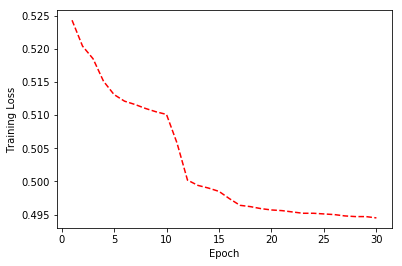
\includegraphics[width = 4.5in]{images/loss.png}
	\caption{Training Loss of ANN} %figure name
\end{center}
\end{figure}

\begin{figure}[tbh]
\begin{center}
	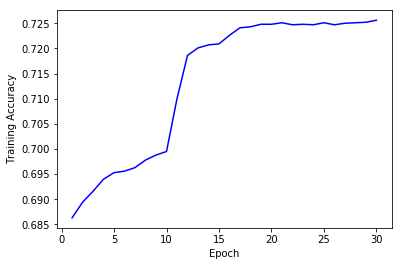
\includegraphics[width = 4.5in]{images/accuracy.png}
	\caption{Training Accuracy of ANN} %figure name
\end{center}
\end{figure}

\clearpage
\section{Receiver Operating Characteristic Curve}
\ac{ROC} curves typically feature true positive rate on the Y axis, and false positive rate on the X axis. This means that the top left corner of the plot is the “ideal” point - a false positive rate of zero, and a true positive rate of one. This is not very realistic, but it does mean that a larger area under the curve (AUC) is usually better.

The “steepness” of \ac{ROC} curves is also important, since it is ideal to maximize the true positive rate while minimizing the false positive rate.


\begin{figure}[tbh]
\begin{center}
	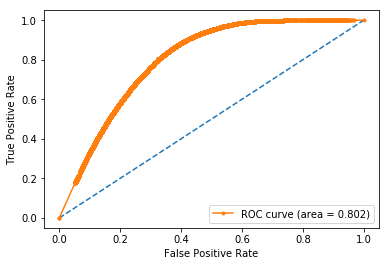
\includegraphics[width = 4.5in]{images/roc.png}
	\caption{\ac{ROC} Curve} %figure name
\end{center}
\end{figure}

\section{Work Schedule}
\begin{figure}[H]
\begin{center}
	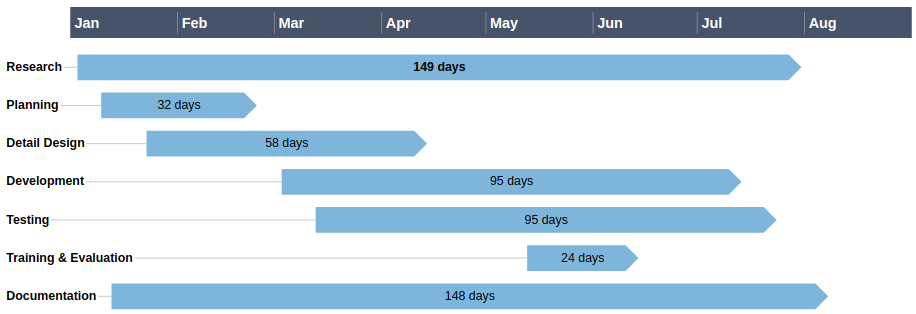
\includegraphics[width = 6in]{images/gantt_.png}
	\caption{Gantt Chart} %figure name
	\label{Gantt Chart} % for referencing
\end{center}
\end{figure}

\chapter{Conclusion}
\section{Conclusion}
The main objective of this project was to develop a module to analyze and identify the questions having same semantic meaning so as to prevent the duplication for Q\&A forums like Quora and which would be able to assist mitigatation of redundancy in answers to support high-quality knowledge base. Using the machine learning techniques on the dataset, the main goal was fulfilled. The project involved understanding the challenges in the collection of relevant features from sentences and designing a system to decide upon the question of duplication of question pairs, and the semantic relatedness of sentences from words.

In conclusion, our projects is capable of adding values to a Q\&A forums and its users as mentioned in the applications.

\section{Future Enhancement}
Regardless of the fulfilment of the project objectives, there are few issues in the process of analysis and decisions, where room for improvements persists. The major limitations of the existing system can be summarized in the following points:

\begin{itemize}
	\item Our system doesn't perform \ac{POS} tagging explicitly. Explicit relationship with adjacent and related words in a phrase, sentence, or paragraph is ignored.
	\item Not designed for \ac{NER}, the subtask of information extraction that seeks to locate and classify named entity mentions in unstructured text into pre-defined categories such as the person names, organizations, locations, medical codes, time expressions, quantities, monetary values, percentages, etc.
	\item Quora's dataset cannot cover the entirety of questions necessary for a machine model to interpret and so, there are cases where the system fails to do so.
\end{itemize}

We, in the field of statistics and machine learning tried to develop theoretical models aiming to predict the behaviour of a certain process, the idea of the quote, ``All models are wrong, but some are useful" is that every single model will be wrong, holds for every machine model, meaning that it will never represent the exact real behaviour. Having said that, even if a model cannot describe exactly the reality, it could be very helpful if it is close enough, where the areas of further improvements and enhancements are presented as follows:

\begin{itemize}
	\item \textbf{Data from multiple Q\&A forums} \\
	Our only source of question pairs is Quora. Collecting data from other sources helps to cover more of the entirety of questions, as one source cannot cover all the questions. This helps to get the complete picture of the situation.
	
	\item \textbf{Perform \acl{POS} Tagging} \\
	Part-of-speech tagging is harder yet more accurate than just having a list of words and their parts of speech, because some words can represent more than one part of speech at different times, and because some parts of speech are complex or unspoken. This is not rare, in natural languages, a large percentage of word-forms are ambiguous.
	
	\item {\textbf{Perform \acl{NER}}} \\
	Classification of named entities that are present in a text into pre-defined categories like “individuals”, “companies”, “places”, “organization”, “cities”, “dates”, “product terminologies” etc. is not implemented in the system, but if performed, it could add a wealth of semantic knowledge to the content and helps to promptly understand the subject of any given text.
\end{itemize}

%Reference
\renewcommand\bibname{References} % Change heading to References
\bibliographystyle{IEEEtran} % to use IEEE Format for referencing
\addcontentsline{toc}{chapter}{References} % to add references in TOC
\bibliography{library} % specify the .bib file containing reference information 

%Comment this Chapter if you do not need to include Appendix.
%\chapter*{Appendix}
%\addcontentsline{toc}{chapter}{Appendix}
%Appendix Text Comes Here

\end{document}
